%2multibyte Version: 5.50.0.2960 CodePage: 1252

\documentclass{beamer}
%%%%%%%%%%%%%%%%%%%%%%%%%%%%%%%%%%%%%%%%%%%%%%%%%%%%%%%%%%%%%%%%%%%%%%%%%%%%%%%%%%%%%%%%%%%%%%%%%%%%%%%%%%%%%%%%%%%%%%%%%%%%%%%%%%%%%%%%%%%%%%%%%%%%%%%%%%%%%%%%%%%%%%%%%%%%%%%%%%%%%%%%%%%%%%%%%%%%%%%%%%%%%%%%%%%%%%%%%%%%%%%%%%%%%%%%%%%%%%%%%%%%%%%%%%%%
\usepackage{amsfonts}
\usepackage{amssymb}
\usepackage{amsmath}
\usepackage{mathpazo}
\usepackage{hyperref}
\usepackage{multimedia}
\usepackage{enumerate}
%\usepackage{newpnts}
\usepackage{graphicx}
\usepackage{booktabs}
\usepackage[labelfont={small},textfont={footnotesize}]{caption}
\usepackage{subfig}
\usepackage{natbib} % already loaded by elsarticle
\usepackage{apalike}
\usepackage{babel}
 \usepackage{appendixnumberbeamer}
% \usepackage{xmpmulti}

\setcounter{MaxMatrixCols}{10}


\newtheorem{acknowledgement}[theorem]{Acknowledgement}
\newtheorem{algorithm}[theorem]{Algorithm}
\newtheorem{axiom}[theorem]{Axiom}
\newtheorem{case}[theorem]{Case}
\newtheorem{claim}[theorem]{Claim}
\newtheorem{conclusion}[theorem]{Conclusion}
\newtheorem{condition}[theorem]{Condition}
\newtheorem{conjecture}[theorem]{Conjecture}
\newtheorem{criterion}[theorem]{Criterion}
\newtheorem{exercise}[theorem]{Exercise}
\newtheorem{notation}[theorem]{Notation}
\newtheorem{proposition}[theorem]{Proposition}
\newtheorem{remark}[theorem]{Remark}
\newtheorem{summary}[theorem]{Summary}
\newenvironment{stepenumerate}{\begin{enumerate}[<+->]}{\end{enumerate}}
\newenvironment{stepitemize}{\begin{itemize}[<+->]}{\end{itemize} }
\newenvironment{stepenumeratewithalert}{\begin{enumerate}[<+-| alert@+>]}{\end{enumerate}}
\newenvironment{stepitemizewithalert}{\begin{itemize}[<+-| alert@+>]}{\end{itemize} }

% Create arg max/min operator
\DeclareMathOperator*{\argmax}{arg\,max}
\DeclareMathOperator*{\argmin}{arg\,min}
\DeclareMathOperator{\E}{\mathbb{E}}

%\input{tcilatex}
\usetheme{Singapore}
\setbeamercovered{transparent=25,highly dynamic}
\setbeamertemplate{itemize subitem}{\tiny\raise1.5pt\hbox{\donotcoloroutermaths$\blacktriangleright$}}
\setlength{\abovecaptionskip}{0pt}
\setlength{\belowcaptionskip}{0pt}
\renewcommand{\theenumi}{\arabic{enumi}}
\renewcommand{\theenumii}{\alph{enumii}} 
% \graphicspath{{C:/Dropbox/Coauthors/Luiggi/SacRatio/Presentations} }

\begin{document}

\title[AIT-Indeterminacy]{Implications for Determinacy with Average Inflation Targeting}
\author[Ahmad]{Yamin Ahmad \inst{1} \and James Murray \inst{2}}
\institute[UW-Whitewater]{\inst{1} University of Wisconsin - Whitewater \and %
						  \inst{2} University of Wisconsin - La Crosse}
\date{\color{red} Society for Nonlinear Dynamics and Econometrics \\ 2023 Symposium \color{black} \\ Orlando, FL, March 16 2023}

\begin{frame}
	\vspace{-1.5cm}
	\titlepage
\end{frame}
%\vspace{-2cm}
%{\titlepage}

\section*{Introduction and Motivation}

\begin{frame}
	\frametitle{Monetary Policy Strategy, August 2020}
	August 27, 2020 \\
	\vspace{1em} 
	Statement on Longer-Run Goals and Monetary Policy Strategy by the FOMC:
	\begin{quotation}
		``In order to anchor longer-term inflation expectations at this level, the Committee seeks to achieve inflation that averages 2 percent over time, and therefore judges that, following periods when inflation has been running persistently below 2 percent, appropriate monetary policy will likely aim to achieve inflation moderately above 2 percent for some time.''
	\end{quotation} 
\end{frame}

\begin{frame}
	\frametitle{August 27, 2020 - Jackson Hole, Wyoming}
	\begin{quotation}
		``... our new statement indicates that we will seek to achieve inflation that \textbf{\textcolor{red}{averages}} 2 percent over time. Therefore, following periods when inflation has been running below 2 percent, appropriate monetary policy will likely aim to achieve inflation moderately above 2 percent for some time. \\
		
		In seeking to achieve inflation that averages 2 percent over time, \textbf{\textcolor{red}{we are not tying ourselves to a particular mathematical formula that defines the average}}. Thus, our approach could be viewed as a flexible form of \textcolor{red}{average inflation targeting}."- Jerome Powell
	\end{quotation} 
\end{frame}

\begin{frame}
	\frametitle{Research Question}
	\textcolor{blue}{Question(s): What is the impact of Average Inflation Targeting - AIT?}
	\begin{itemize}
		\item How is the `average' measure of inflation constructed?
		\begin{itemize}
			\item Is it an (weighted) average of past inflation terms?
			\item Is it an (weighted) average of expected future inflation?
			\item Is the measure a hybrid?
		\end{itemize}
		\item \setlength\itemsep{1em} Are there implications for (in)determinacy? 
		\item Does the length of the `window' used to construct the average impact stability?
		\item If we consider a hybrid, what happens if the window lengths (forward vs backwards) are asymmetric? 
		\item What is the impact of a monetary policy shock under AIT?
	\end{itemize}
\end{frame}

\begin{frame}
	\frametitle{Literature}
	\textcolor{purple}{AIT}
	\begin{itemize}
		\item Welfare Implications and Stability - \cite{budianto2020}, \cite{eo2020}, \cite{piergallini2022}
		\item Impact on Inflation expectations - \cite{coibion2020}, \cite{hoffmann2022}
		\item Impact on boundedly rational expectations - \cite{honka2021}, \cite{budianto2020}
	\end{itemize}
	\textcolor{purple}{Monetary policy rules}
	\begin{itemize}
		\item Indeterminacy and Stability of policy rules - \cite{clarida2000monetary}, \cite{lubik2004testing}, \cite{evans2005monetary}, \cite{nessen2005}, \cite{castelnuovo2015monetary}, \cite{mertens2019tying}, \cite{svensson2020monetary}
	\end{itemize}
\end{frame}

\section*{Design and Framework}

\begin{frame}
	\frametitle{New Keynesian Framework}
	\textcolor{purple}{There are 3 key equations of interest in the NK framework with monetary policy}
	\vspace{1em}
	\begin{itemize}
		\setlength{\itemsep}{1em}
		\item The key equations include:
		\begin{itemize}
			\setlength{\itemsep}{1em}
			\item The \textcolor{red}{IS Curve} - derived from the Household's utility maximization problem
			\item The \textcolor{red}{Phillips Curve} - derived from the Firm's problem
			\item The \textcolor{red}{monetary policy rule} (e.g. a Taylor-type rule)
		\end{itemize}
		\item We log-linearize the model around the (long-run) steady state.
	\end{itemize}
\end{frame}

\begin{frame}
	\frametitle{New Keynesian Framework}
	\begin{itemize}
		\item The IS Equation:
		\begin{equation}\label{eq:ISe}
			x_t = x_{t+1|t}^e - \frac{1}{\sigma} \left( r_t - \pi_{t+1|t}^e  - r^n  \right) + \xi_t^{x},
		\end{equation}
		\item We assume that a fraction of agents, $\lambda\in[0,1)$, form na\"ive expectations, so aggregate expectations are given by,
		\begin{equation}
			\begin{array}{c}
				x_{t+1}^e = \lambda x_t + (1-\lambda) \E_t x_{t+1}, \\ [1.5pc]
				\pi_{t+1}^e = \lambda \pi_t + (1-\lambda) \E_t \pi_{t+1}. \\
			\end{array}
		\end{equation}
		\item Expectations are fully rational when $\lambda=0$. We allow $\lambda \neq 0$.
	\end{itemize}
\end{frame}

\begin{frame}
	\frametitle{New Keynesian Framework}
	\begin{itemize}
		\item The Phillips Curve: 
		\begin{equation}\label{eq:PhillipsCurvee}
			(\pi_t - \pi^*) = \beta (\pi_{t+1|t}^e - \pi^*) + \kappa x_t + \xi_t^{\pi},
		\end{equation}
		\item The monetary policy rule:
		\begin{align}\label{eq:TaylorRule}
			r_t &= (1-\rho_r)(r^n + \pi^*) + \rho_r r_{t-1} \nonumber \\
				& + (1-\rho_r) \left[ \psi_\pi (\color{red}\pi_t^A \color{black} - \pi^*) + \psi_x x_t \right] + \epsilon_t^{r},
		\end{align}
	\end{itemize}
\end{frame}

\begin{frame}
	\frametitle{Average Inflation Targeting}
	\begin{itemize}
		\setlength{\itemsep}{1em}
		\item We assume that monetary policy targets an average value of inflation over a target window that may include backward- and forward-looking terms for inflation. 
		\item The average inflation target is:
		\begin{equation}
			\pi_t^A = \gamma \pi_t^B + (1-\gamma) \pi_t^F,
		\end{equation}
		where $\gamma \in [0,1]$ is the relative weight given to past average inflation, $\pi_t^B$, versus expected future average inflation, $\pi_t^F$.
	\end{itemize}
\end{frame}

\begin{frame}
	\frametitle{Backwards window for AIT}
	\begin{itemize}
		\setlength{\itemsep}{1em}
		\item The past average inflation, $\pi_t^B$, is given by:
		\begin{equation}\label{eq:backward}
			\pi_t^B = \delta_B \pi_t + (1-\delta_B) \pi_{t-1}^B,
		\end{equation}
		where $\delta_B \in (0,1)$ is the weight given to the most recent observation.
		\item Substituting recursively, we obtain:
		\begin{equation*}\label{eq:backward_all}
			\pi_t^B = \delta_B \sum_{j=0}^{\infty} (1-\delta_B)^j \pi_{t-j},
		\end{equation*}
		where $\sum_j \delta_B (1-\delta_B)^j=1$, and $\lim_{j \to \infty} \delta_B (1-\delta_B)^j=0$.
		\item A weight of $\delta_B$ approximates monetary policy behavior using an equally-weighted finite window of length $1 / \delta_B$ periods.
	\end{itemize}
\end{frame}

\begin{frame}
	\frametitle{Forward window for AIT}
	\begin{itemize}
		\setlength{\itemsep}{1em}
		\item Similarly, the forward window includes expected future average inflation, $\pi_t^F$:
		\begin{align}\label{eq:forward}
			\pi_t^F &= \delta_F \E_t \pi_{t+1} + (1-\delta_F) \E_t \pi_{t+1}^F \\
			\implies \pi_t^F &= \delta_F \sum_{j=0}^{\infty} (1-\delta_F)^j \E_t \pi_{t+1+j} \nonumber
		\end{align}
		where $\delta_F \in (0,1)$ is the weight given to next period's expected inflation and $\sum_j \delta_F (1-\delta_F)^{j}=1$, and $\lim_{j \to \infty} \delta_F (1-\delta_F)^j=0$.
		\item Similarly, $1/ \delta_F$ approximates the length of an equally-weighted finite forward-looking window.
	\end{itemize}
\end{frame}

\begin{frame}
	\frametitle{Summary of Key Parameters}
	\begin{itemize}
		\item We vary the parameters below and explore the implications for determinacy: 
		\begin{itemize}
			\item  $\left\{\delta_B, \delta_F \right\}$ - the weights on the previous/next period's (expected) inflation
			\item $\gamma$ - the relative weight on past vs expected future inflation
			\item $\lambda$ - the share of the population that form na\"ive expectations
			\item  $\left\{\psi_\pi, \psi_x \right\}$ - the weights on the inflation and output gap terms in the policy rule
			\item $\rho_r$ - the persistence of monetary policy
		\end{itemize}
		\item Note that a standard Taylor-type rule emerges as a special case with $\gamma=1.0$ and $\delta_B=1.0$.
	\end{itemize}
\end{frame}

\section*{Methodology}

\begin{frame}[allowframebreaks]
	\frametitle{Key Model Equations}
	\begin{enumerate}
		\item The IS Equation:
		\begin{equation*}
			x_t = x_{t+1|t}^e - \frac{1}{\sigma} \left( r_t - \pi_{t+1|t}^e  - r^n  \right) + \xi_t^{x},
		\end{equation*}
		\item The Phillips Curve: 
		\begin{equation*}
			(\pi_t - \pi^*) = \beta (\pi_{t+1|t}^e - \pi^*) + \kappa x_t + \xi_t^{\pi},
		\end{equation*}
		\item Evolution of the expected output gap
		\begin{equation*}
			x_{t+1}^e = \lambda x_t + (1-\lambda) \E_t x_{t+1}
		\end{equation*}
		\item Evolution of the expected inflation
		\begin{equation*}
			\pi_{t+1}^e = \lambda \pi_t + (1-\lambda) \E_t \pi_{t+1}
		\end{equation*}
		\item The monetary policy rule:
		\begin{align*}
			r_t &= (1-\rho_r)(r^n + \pi^*) + \rho_r r_{t-1} \nonumber \\
			& + (1-\rho_r) \left[ \psi_\pi (\color{red}\pi_t^A \color{black} - \pi^*) + \psi_x x_t \right] + \epsilon_t^{r},
		\end{align*}
		\item The average inflation target:
		\begin{equation*}
			\pi_t^A = \gamma \pi_t^B + (1-\gamma) \pi_t^F,
		\end{equation*}
		\item Past average inflation:
		\begin{equation*}
			\pi_t^B = \delta_B \pi_t + (1-\delta_B) \pi_{t-1}^B,
		\end{equation*}
		\item Expected future average inflation:
		\begin{align*}
			\pi_t^F &= \delta_F \E_t \pi_{t+1} + (1-\delta_F) \E_t \pi_{t+1}^F
		\end{align*}
	\end{enumerate}
\end{frame}

\begin{frame}
	\frametitle{Our Approach}
	\begin{itemize}
		\setlength{\itemsep}{1em}
		\item Following \citet{sims2002}, the model can be expressed as:
		\begin{equation}
			\Gamma_0 y_t = \Gamma_1 y_{t-1} + \Psi z_t + \Pi \eta_t
		\end{equation}
		where $y_t$ is a vector that includes $x_t$, $\pi_t$, $r_t$, $\pi_t^A$, $\pi_t^B$, and $\pi_t^F$; $z_t$ is a vector of the shocks, $\xi_t^x$, $\xi_t^\pi$, and $\xi_t^r$; and $\eta_t \equiv y_t - E_{t-1} y_t$ equals the ex-post rational expectations forecast errors. 
		\item We use the method in \citet{sims2002} to explore regions of indeterminacy.
		\begin{itemize}
			\item i.e. do the rank conditions hold for our system of equations?
		\end{itemize}
	\end{itemize}
\end{frame}

\begin{frame}
	\frametitle{Calibration}
	\begin{table}[htp]
		\begin{center}
			\vspace*{-1pc}\begin{tabular}{lcr}
				Description & Parameter & Value \\ \hline
				Discount rate (quarterly) & $\beta$ & 0.99 \\
				Inverse intertemporal elasticity & $\sigma$ & 0.72 \\
				Phillips curve coefficient & $\kappa$ & 0.178 \\
				Steady state inflation rate (quarterly) & $\pi^*$ & 0.005 \\ [0.25pc]
				\hline \\ [-0.25pc]
				Baseline Parameters & Parameter & Value(s) \\ \hline
				AIT weight past inflation & $\gamma$ & $\left\{ 0.0, 0.25 \right\}$ \\
				Backward-looking weight & $\delta_B$ & 1.0 \\
				Monetary policy: average inflation & $\psi_\pi$ & 1.5 \\
				Monetary policy: output gap & $\psi_x$ & 0.5 \\
				Monetary policy: persistence & $\rho_r$ & 0.0 \\ \hline
			\end{tabular}
		\end{center}
%	\captionsetup{justification=centering}
%	\caption{Parameter Calibrations}\label{tb:parms}
	\end{table}
\end{frame}

\section*{Results}

\begin{frame}
	\frametitle{Regions of Determinacy for Forward Looking Windows}	
	\begin{center}		
		\begin{figure}%
			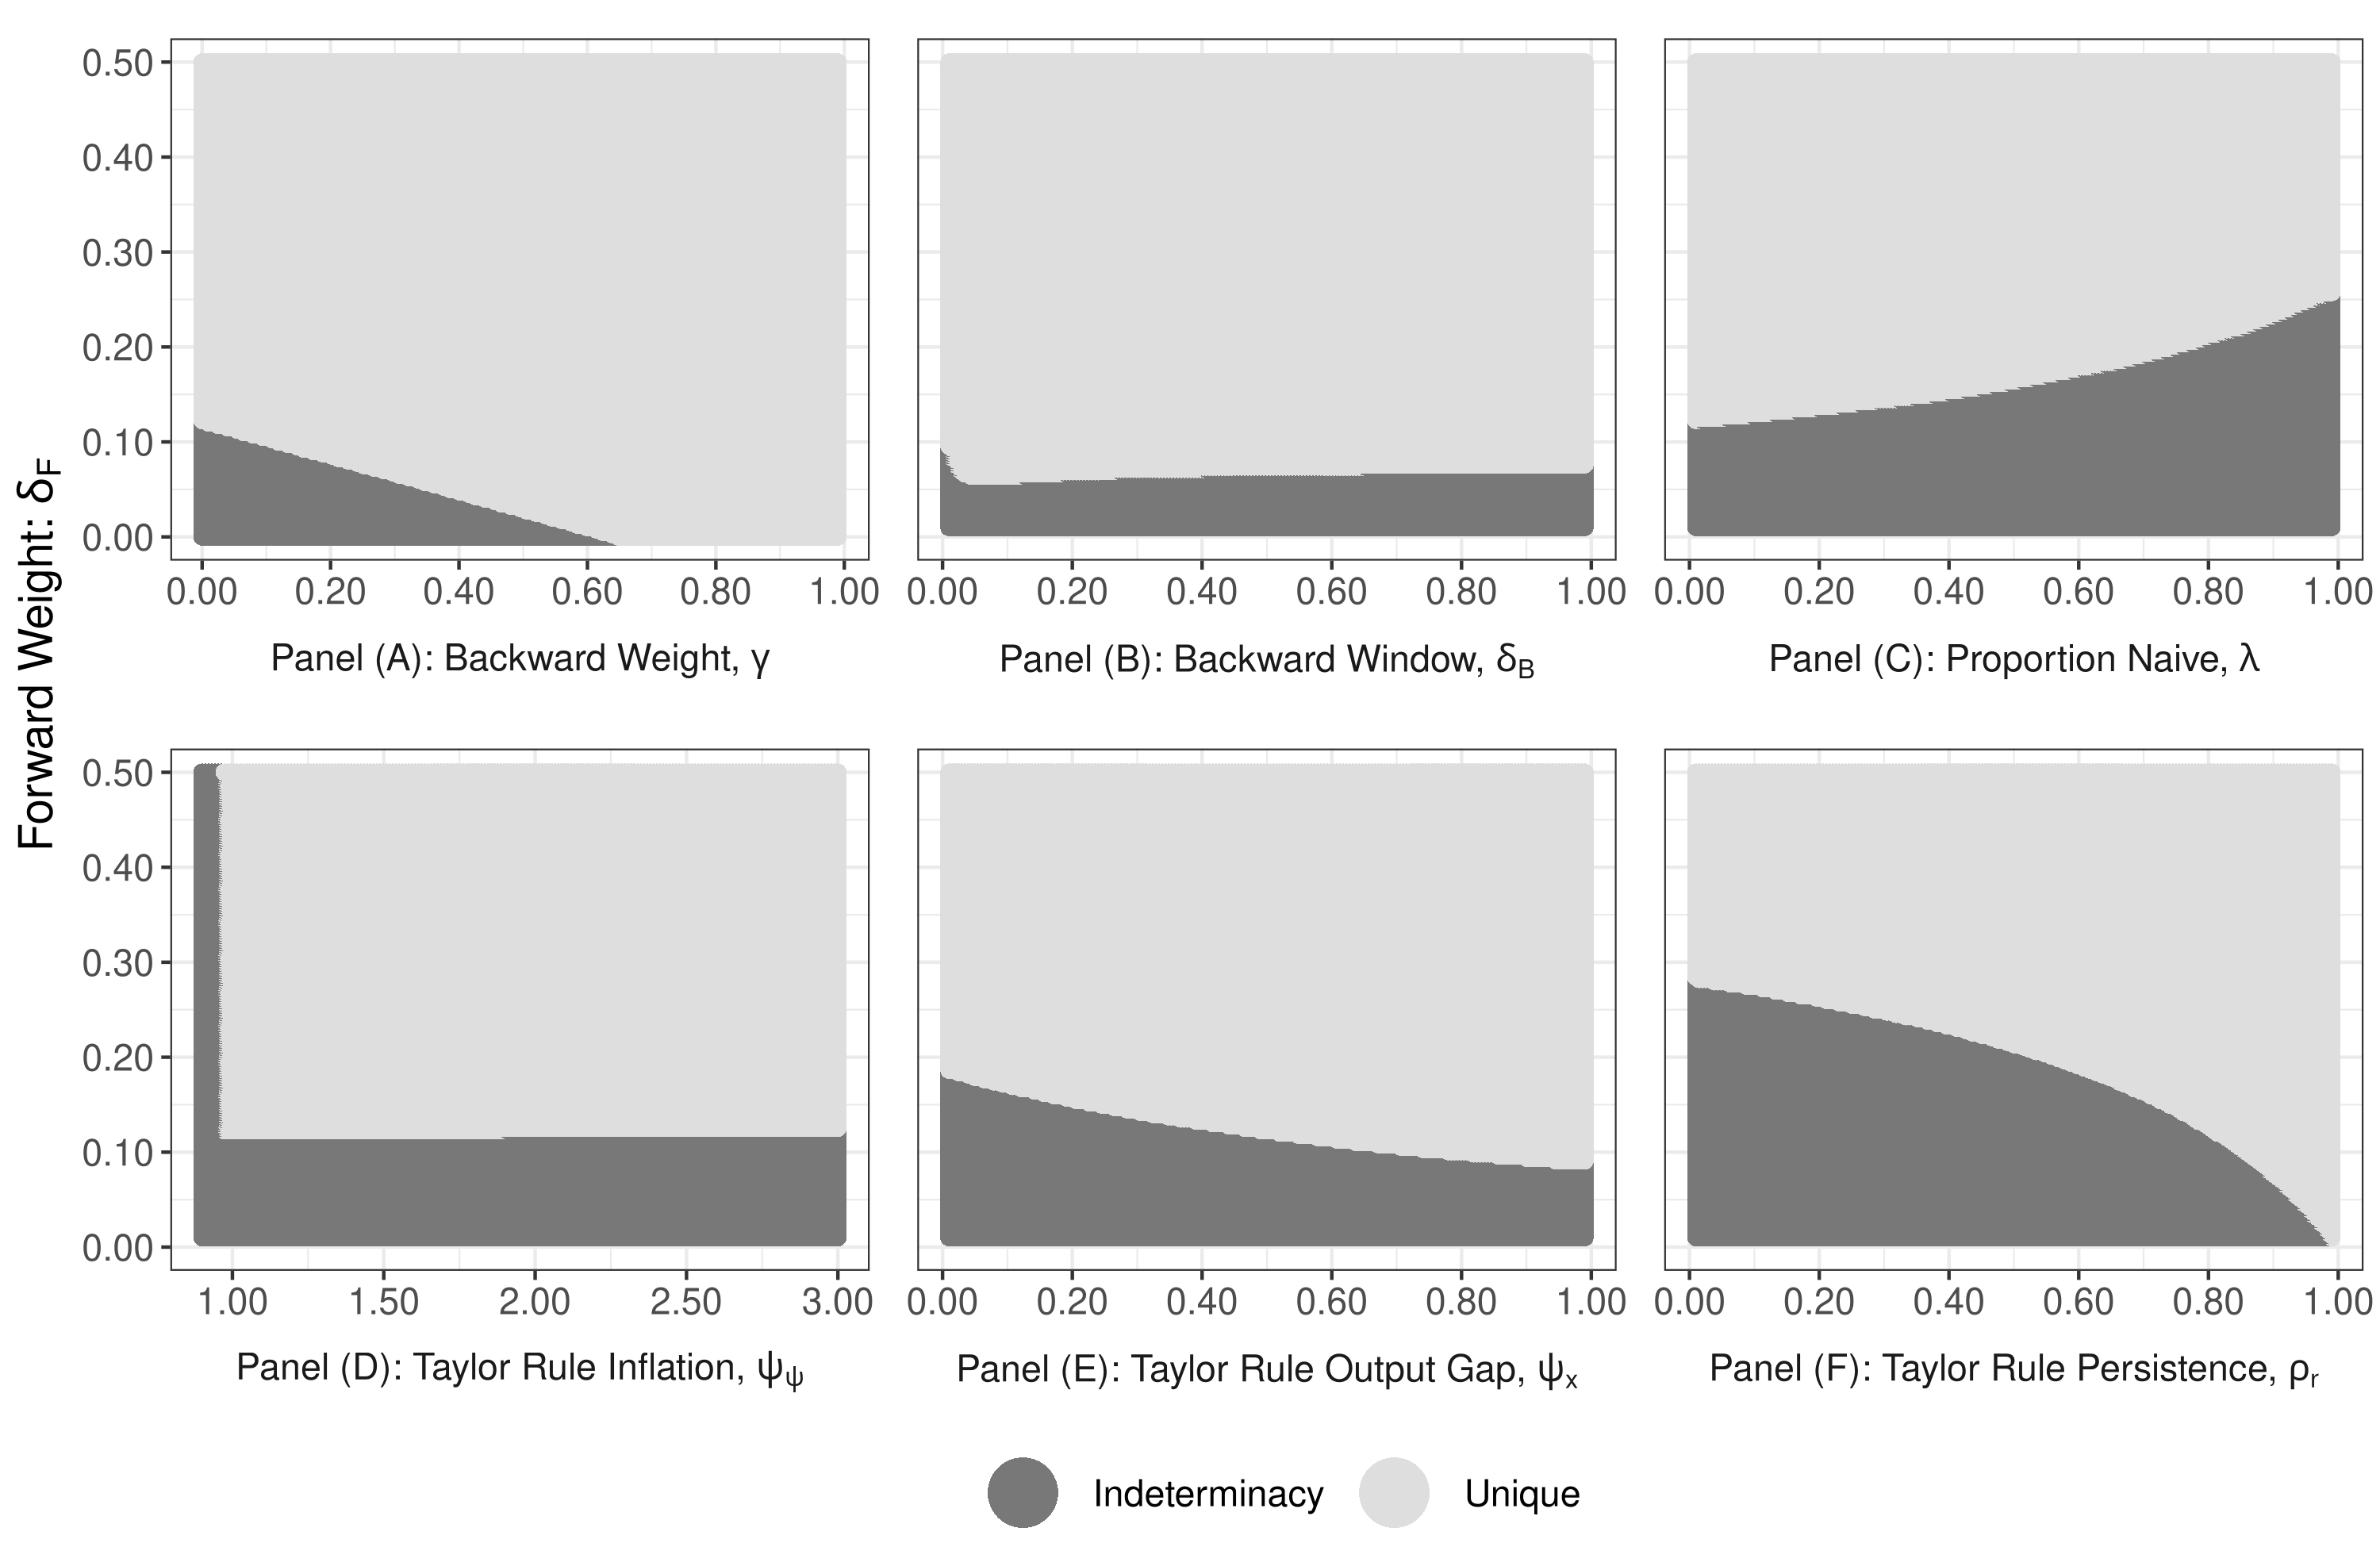
\includegraphics[width=\textwidth,height=0.7\textheight,keepaspectratio]{../code/determinacy_notitle.png}
			\caption{{\tiny In Panel (B), $\gamma = 0.25$, implying a 25\% weight given to the backward-looking window. In all other panels, $\gamma =0$, implying purely forward-looking windows.}}
%			\vspace*{3pc}\hspace*{2pc}\parbox{0.9\textwidth}{\small{
%			Notes: In Panel (B), $\gamma = 0.25$, implying a 25\% weight given to the backward-looking window. In all other panels, $\gamma =0$, implying purely forward-looking windows.}
		\end{figure}% 
	\end{center}%
\end{frame}

\begin{frame}
	\frametitle{Varying the relative weight on past inflation, $\gamma$}	
	\begin{center}		
		\begin{figure}%
			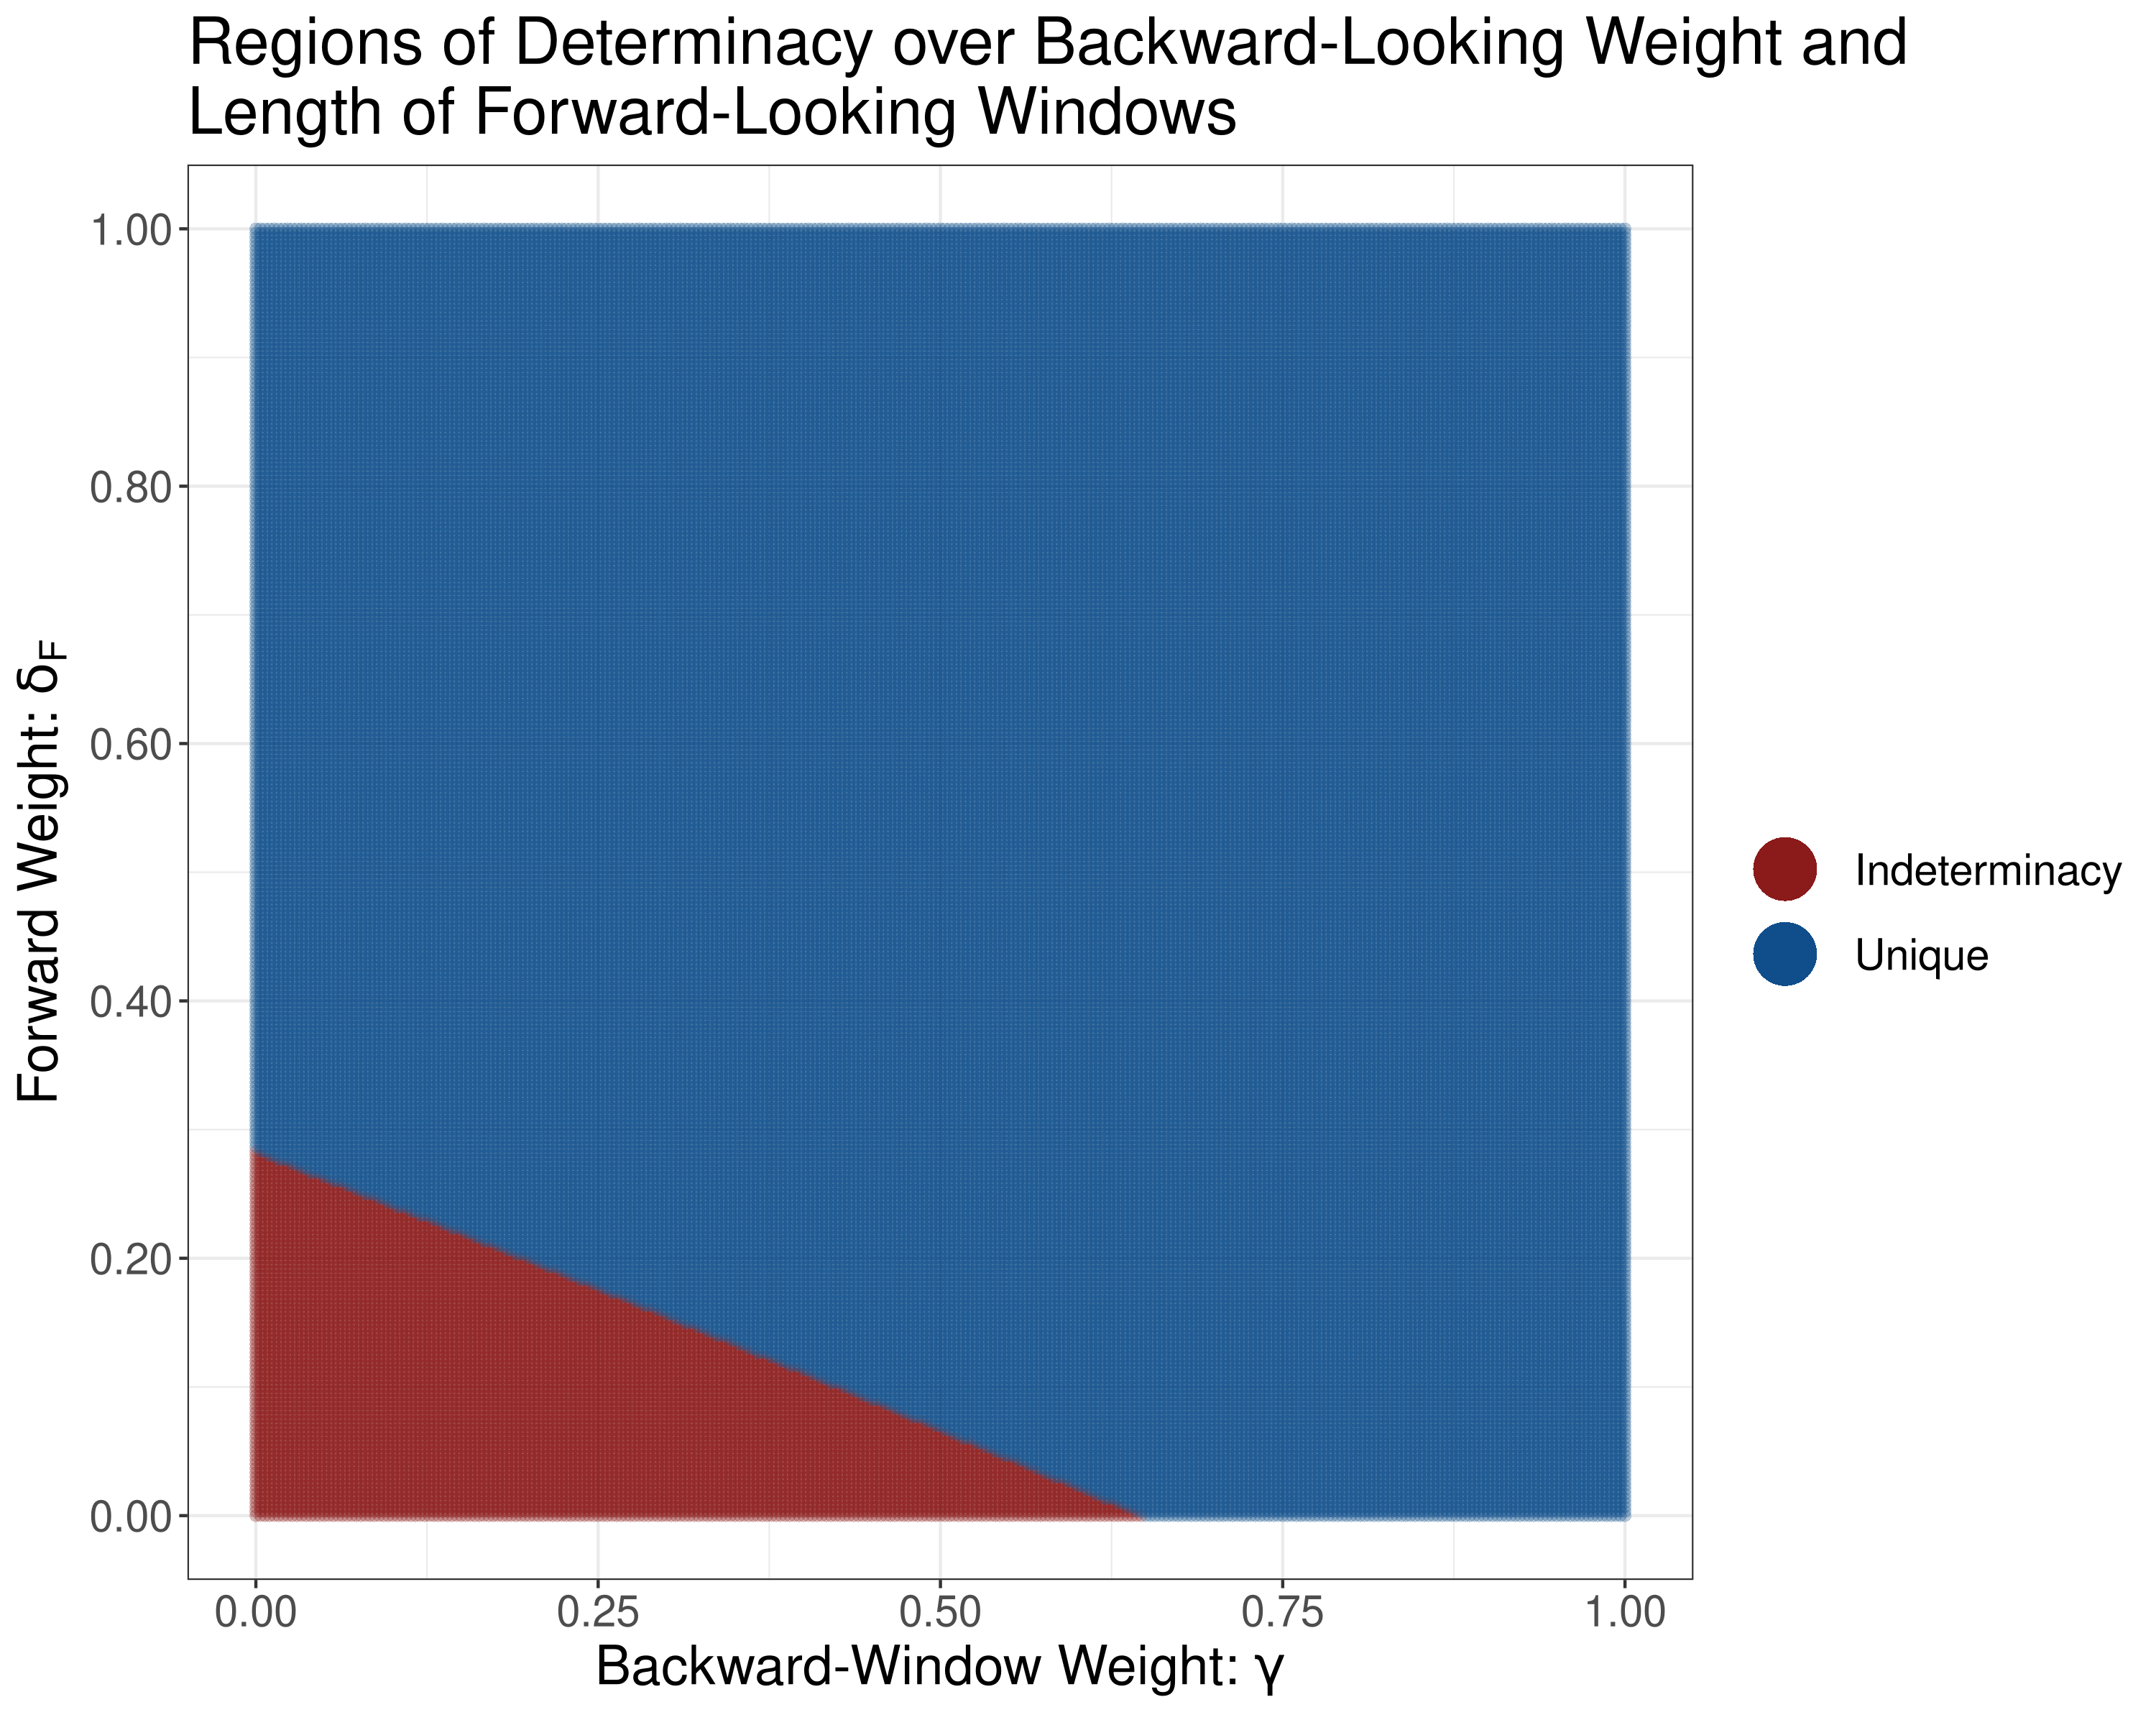
\includegraphics[width=\textwidth,height=0.5\textheight,keepaspectratio]{../code/gamma_deltaF.png}
		\end{figure}% 
		\end{center}%
		\begin{enumerate}
			\setlength{\itemsep}{1em}
			\item In panel (A), $\delta_F =0.28$ is the smallest value that delivers determinacy in this scenario (the largest possible forward-looking window is approximately 3.57 quarters).
		\end{enumerate}
\end{frame}

\begin{frame}
	\frametitle{Varying the relative weight on past inflation, $\gamma$}	
	\begin{center}		
		\begin{figure}%
			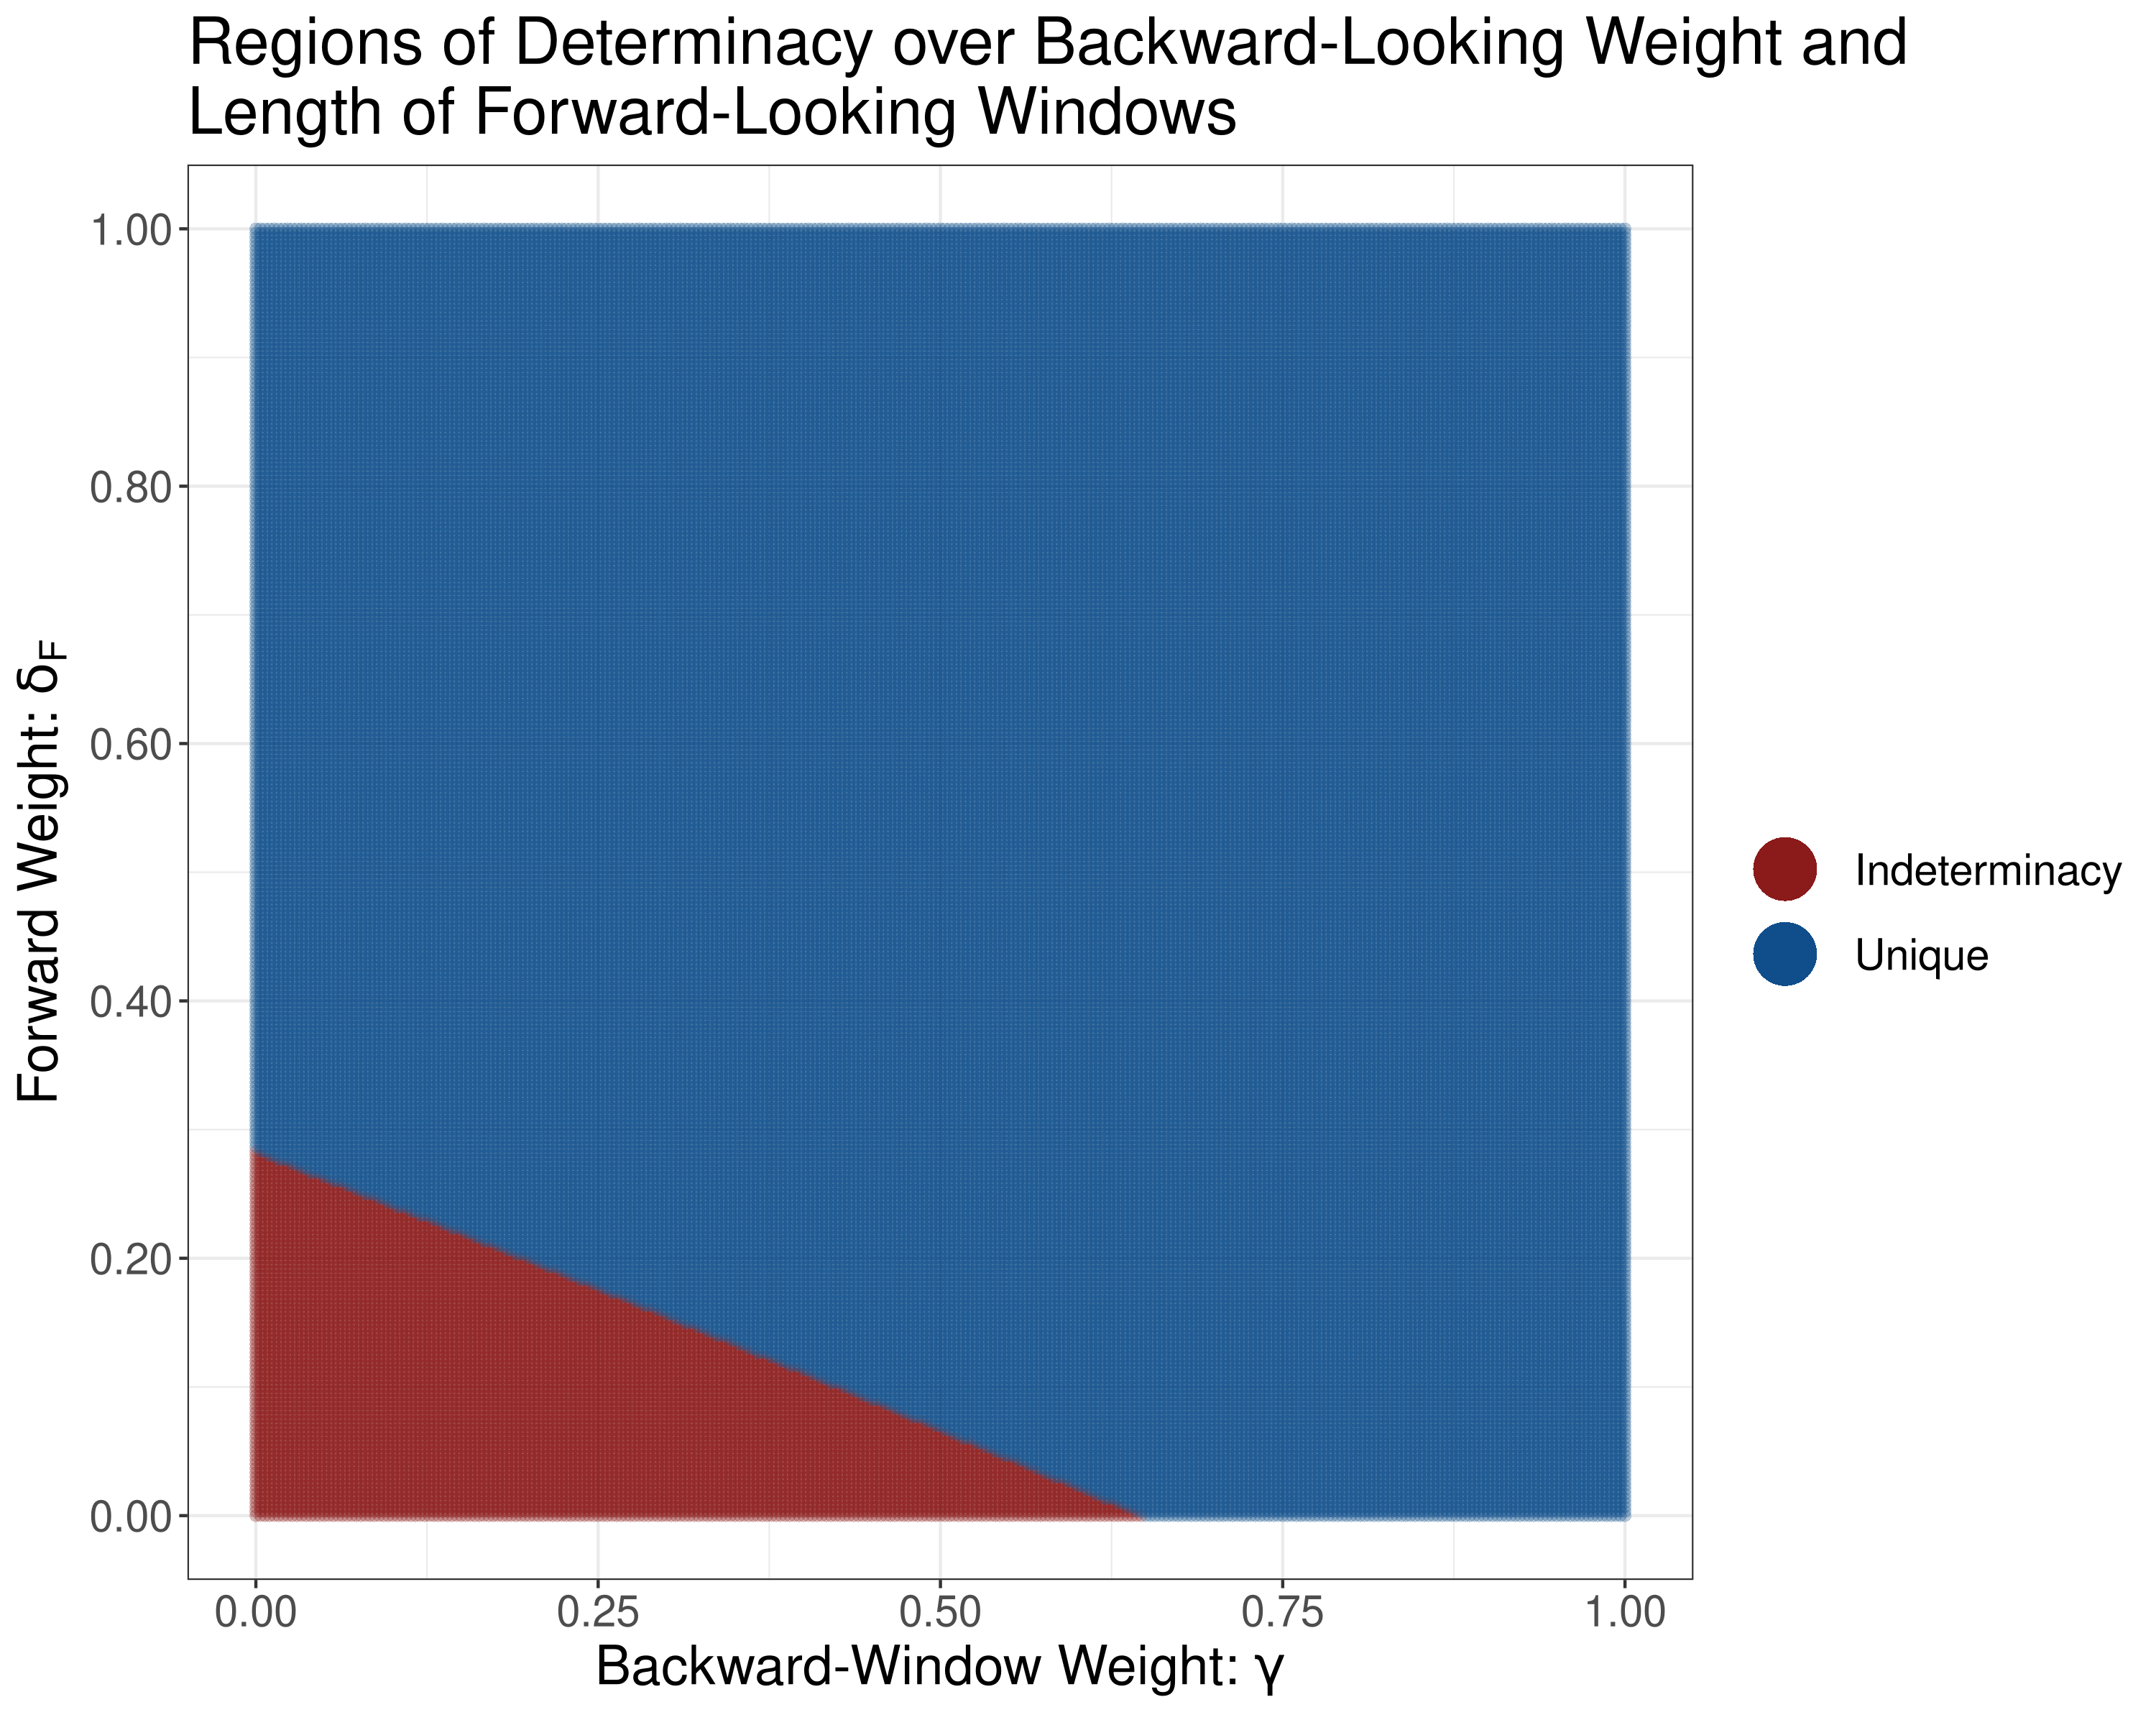
\includegraphics[width=\textwidth,height=0.5\textheight,keepaspectratio]{../code/gamma_deltaF.png}
		\end{figure}% 
	\end{center}%
	\begin{enumerate}
		\setcounter{enumi}{1}
		\setlength{\itemsep}{1em}
		\item When $\gamma \geq 0.63$, all possible forward-looking windows yield determinate solutions. 
		\begin{itemize}
			\item This implies, though, that the target window has at least a 63\% weight on the current inflation rate, and therefore at most a 37\% weight on future inflation.
		\end{itemize}
	\end{enumerate}
\end{frame}

\begin{frame}
	\frametitle{Varying the backward-window weight, $\delta_B$}	
	\begin{center}		
		\begin{figure}%
			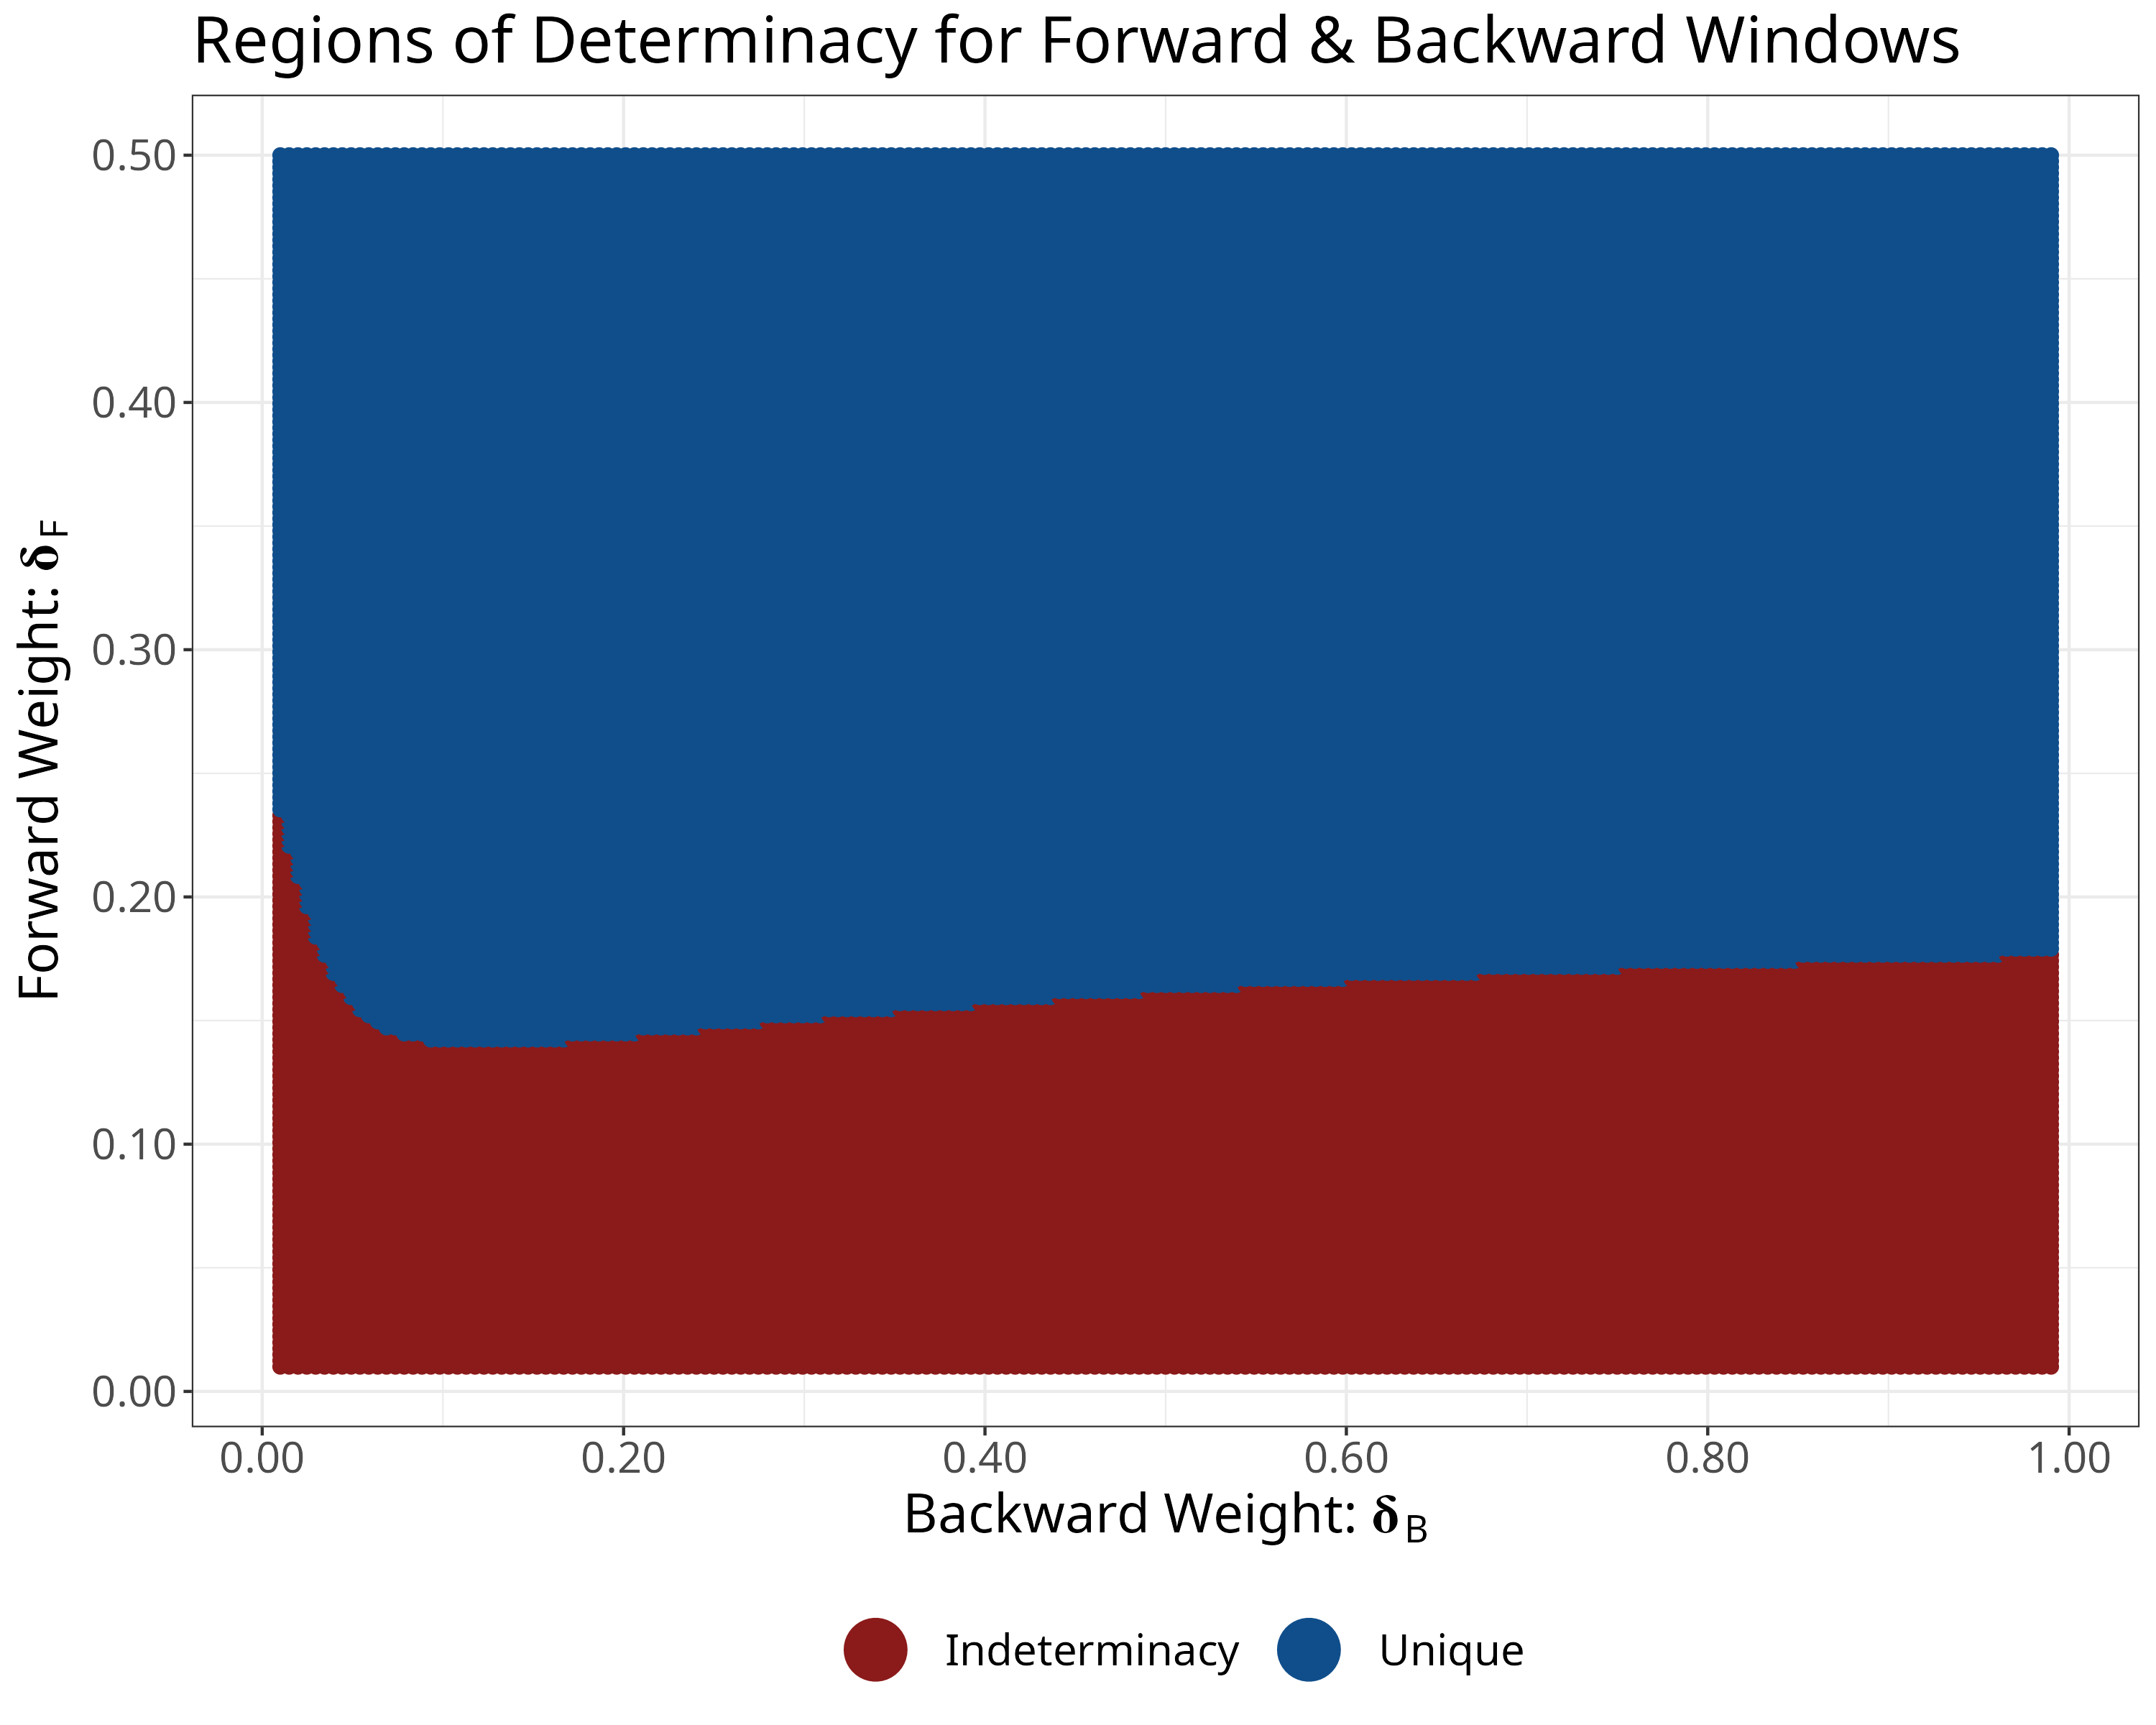
\includegraphics[width=\textwidth,height=0.5\textheight,keepaspectratio]{../code/deltab_deltaF.png}
		\end{figure}% 
	\end{center}%
	\begin{enumerate}
		\setcounter{enumi}{2}
		\setlength{\itemsep}{1em}
		\item The minimal combinations of values for $\delta_B$ and $\delta_F$ that achieve determinacy are each 0.14, implying the longest the forward-looking and backward-looking windows can be are approximately 7.14 quarters.
	\end{enumerate}
\end{frame}

\begin{frame}
	\frametitle{Varying the Proportion of na\"ive expectations, $\lambda$}	
	\begin{center}		
		\begin{figure}%
			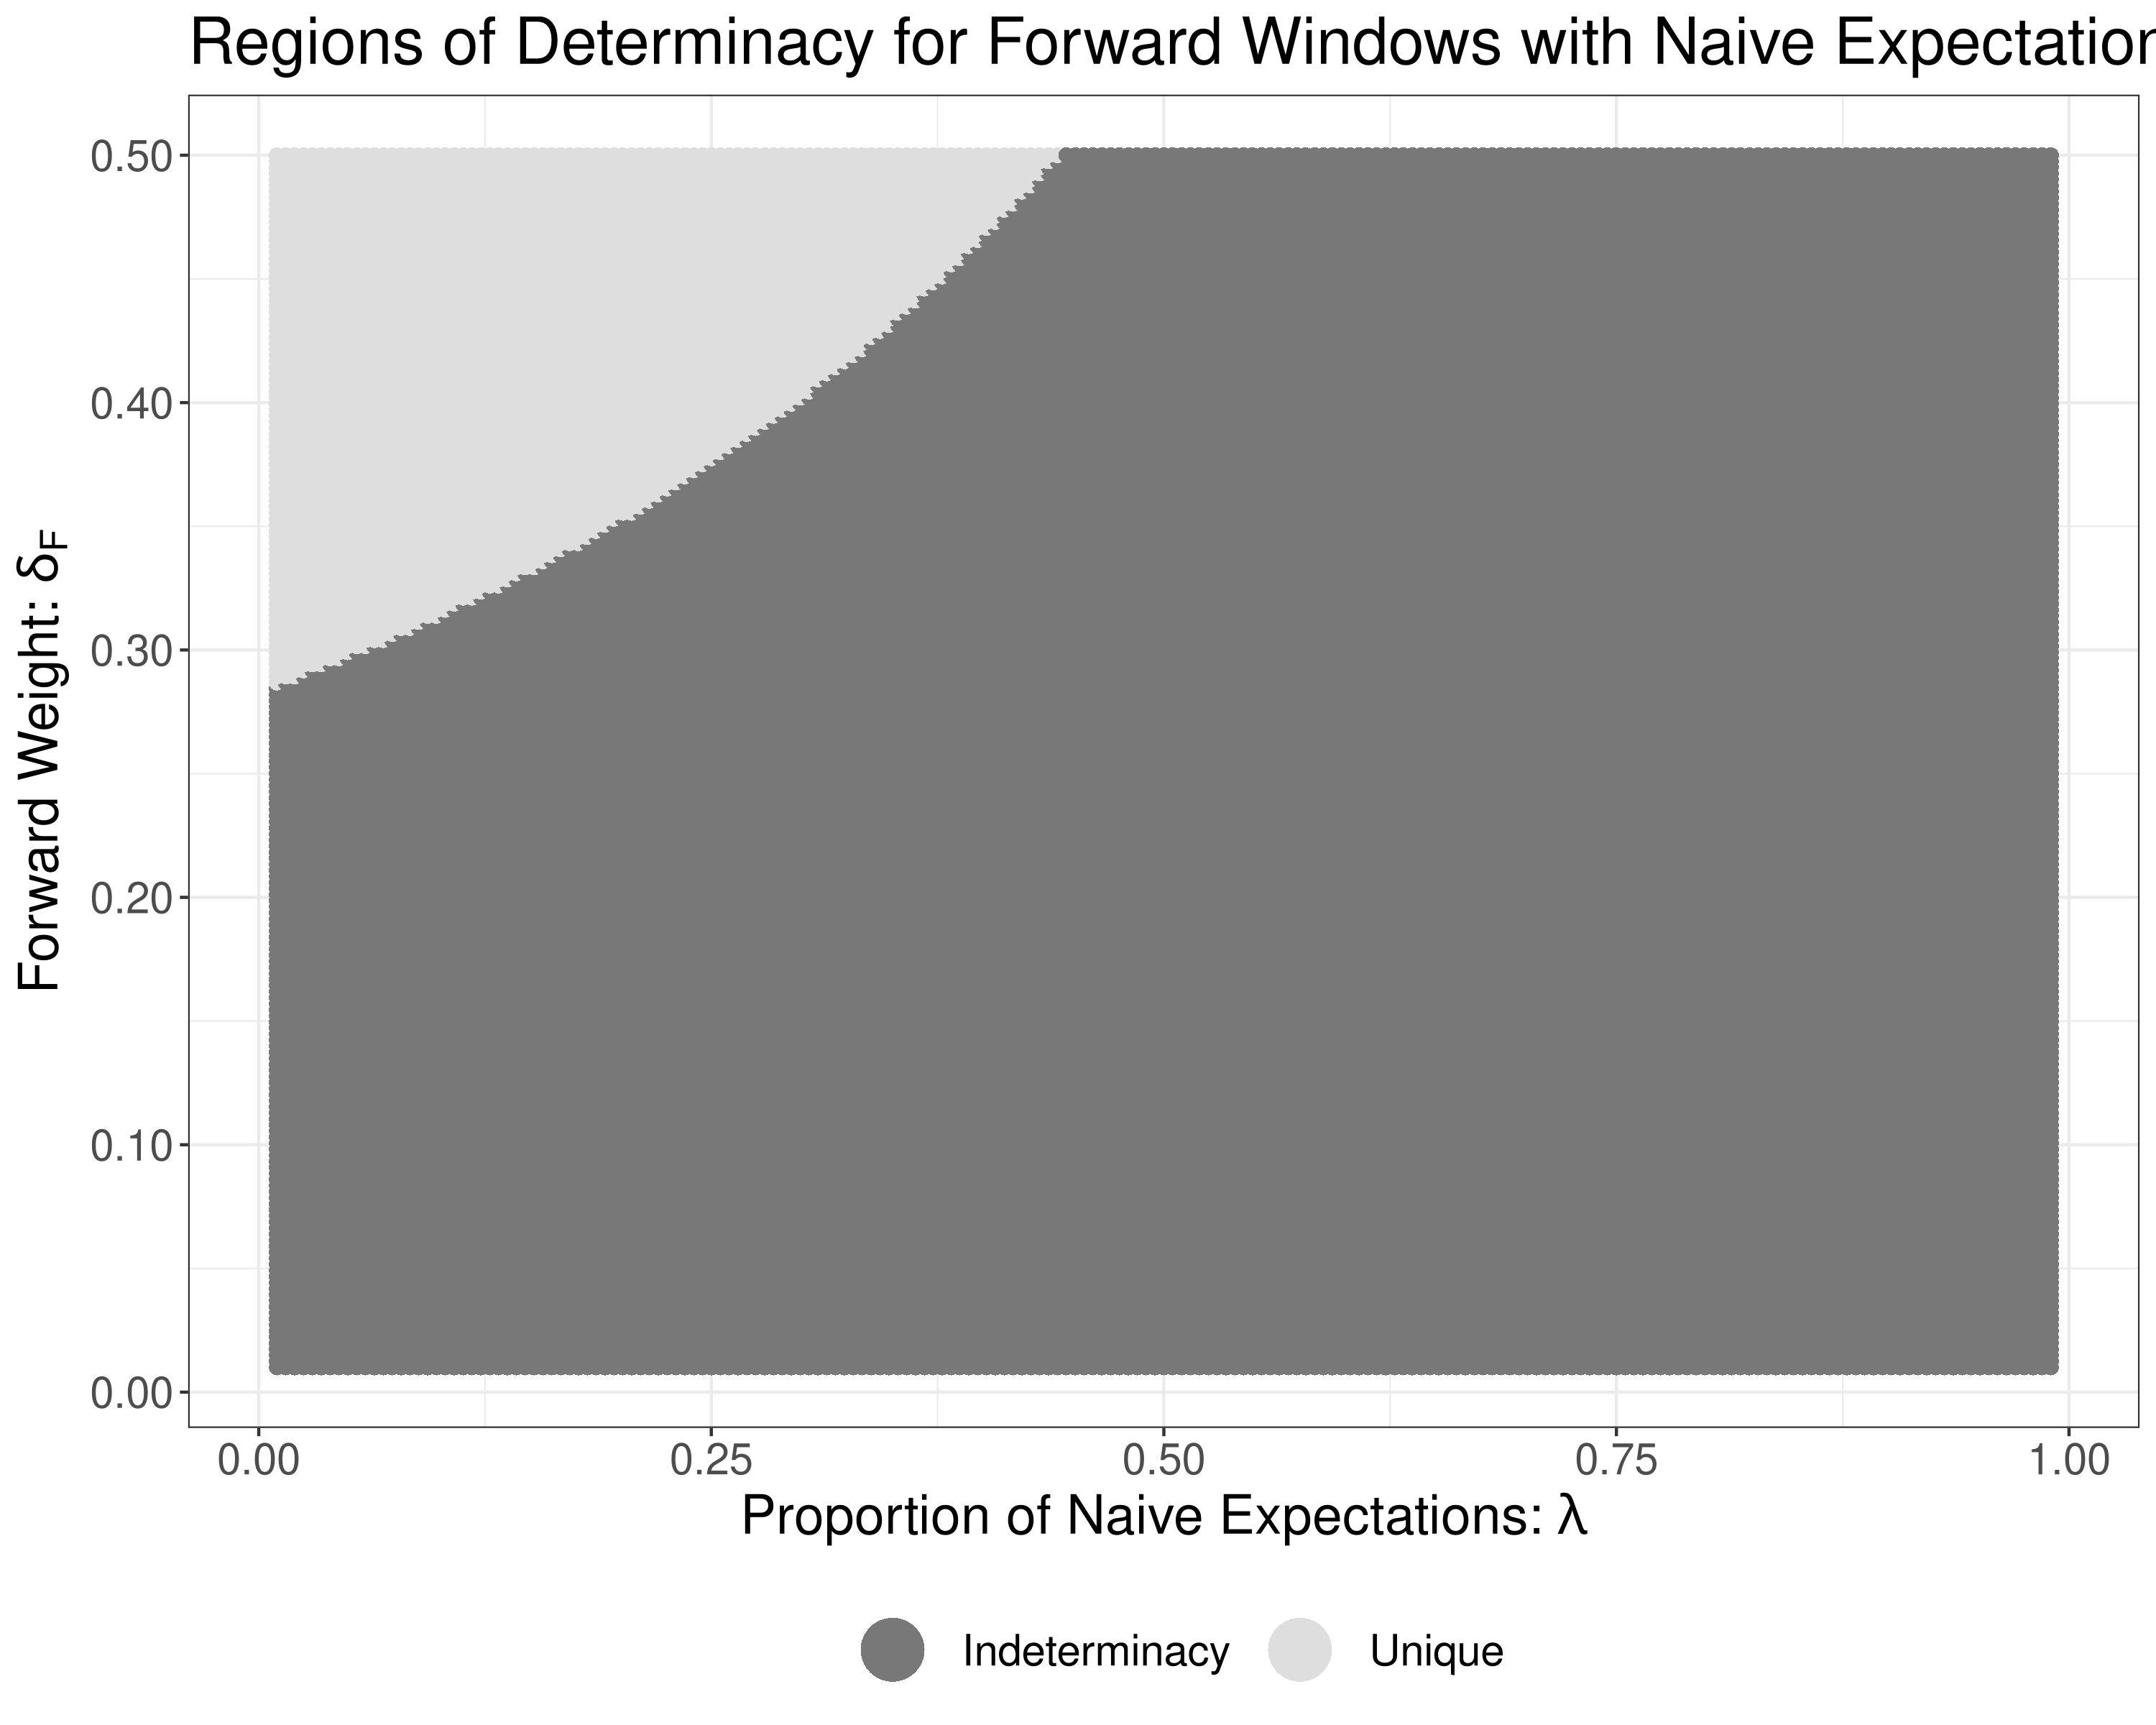
\includegraphics[width=\textwidth,height=0.6\textheight,keepaspectratio]{../code/lambda_deltaF.png}
		\end{figure}% 
	\end{center}%
	\begin{enumerate}
		\setcounter{enumi}{3}
		\setlength{\itemsep}{1em}
		\item When more than 40\% of agents form na\"ive expectations, no purely forward-looking window for AIT leads to determinacy.
	\end{enumerate}
\end{frame}

\begin{frame}
	\frametitle{Varying the weight on the inflation term, $\psi_\pi$}	
	\begin{center}		
		\begin{figure}%
			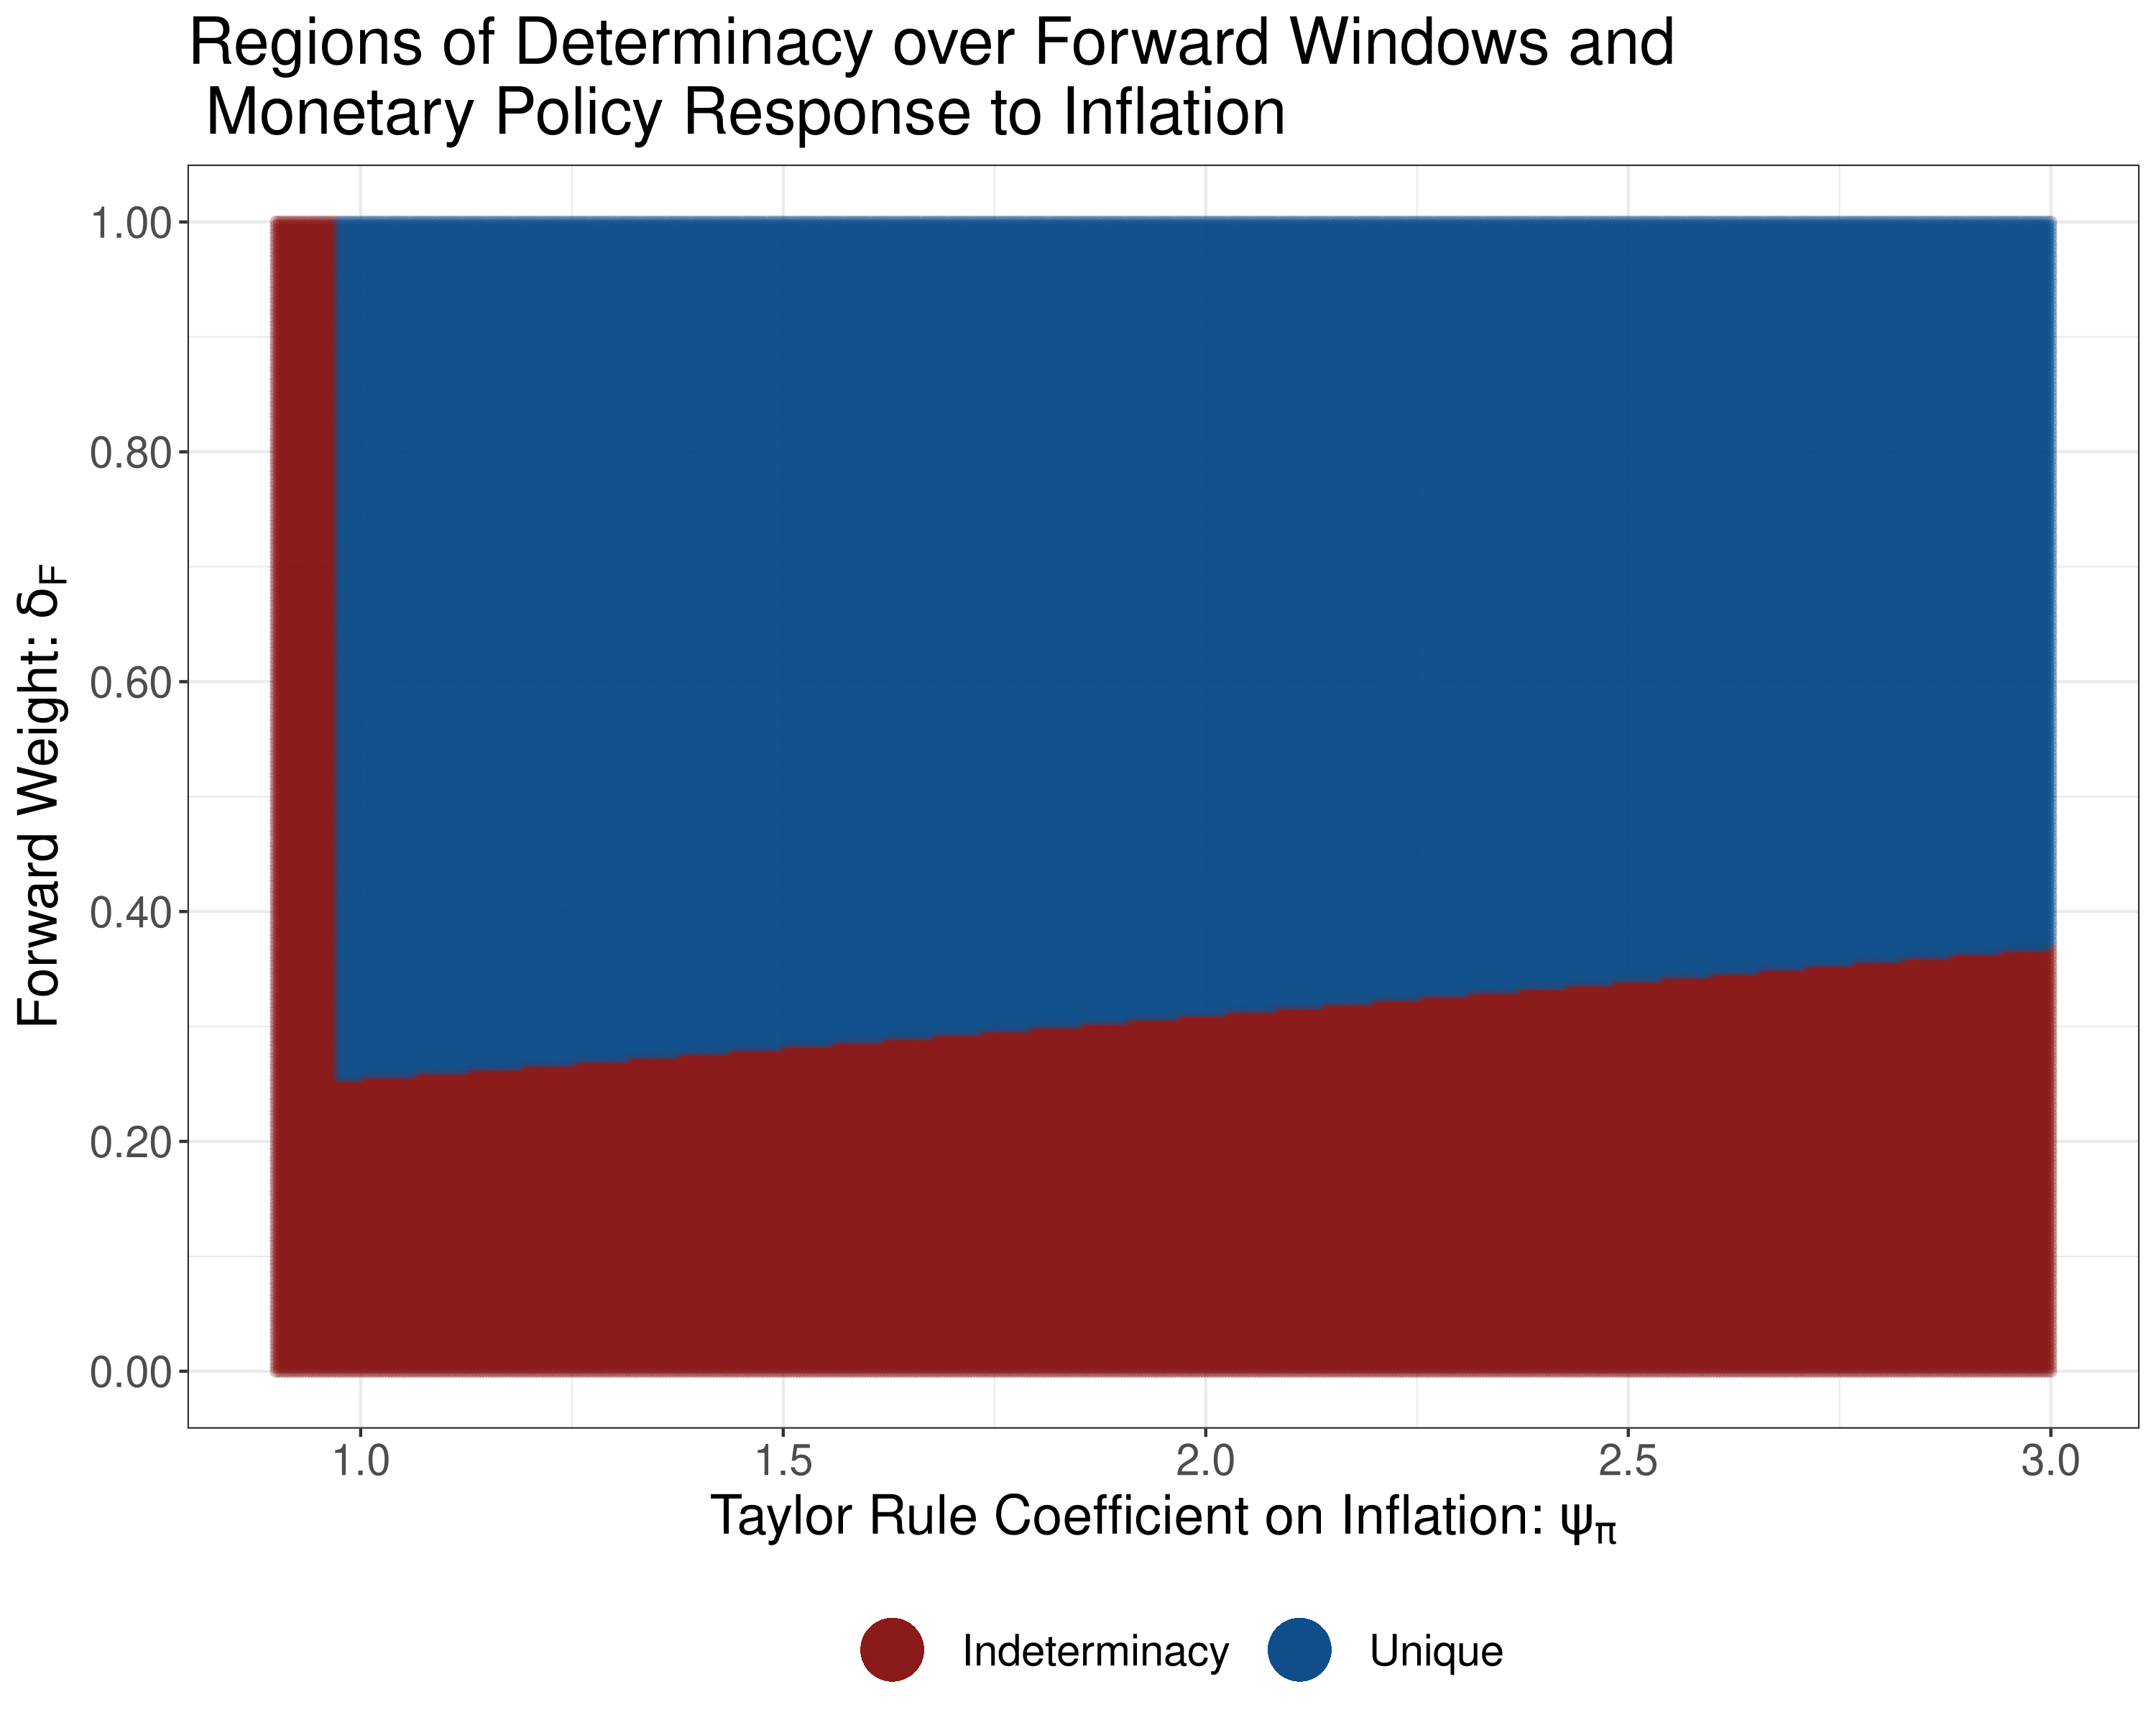
\includegraphics[width=\textwidth,height=0.6\textheight,keepaspectratio]{../code/pi_deltaF.png}
		\end{figure}% 
	\end{center}%
	\begin{enumerate}
		\setcounter{enumi}{4}
		\setlength{\itemsep}{1em}
		\item In general, a larger response to inflation leads to more restrictive (shorter) forward windows
	\end{enumerate}
\end{frame}

\begin{frame}
	\frametitle{Varying the weight on the output-gap term, $\psi_x$}	
	\begin{center}		
		\begin{figure}%
			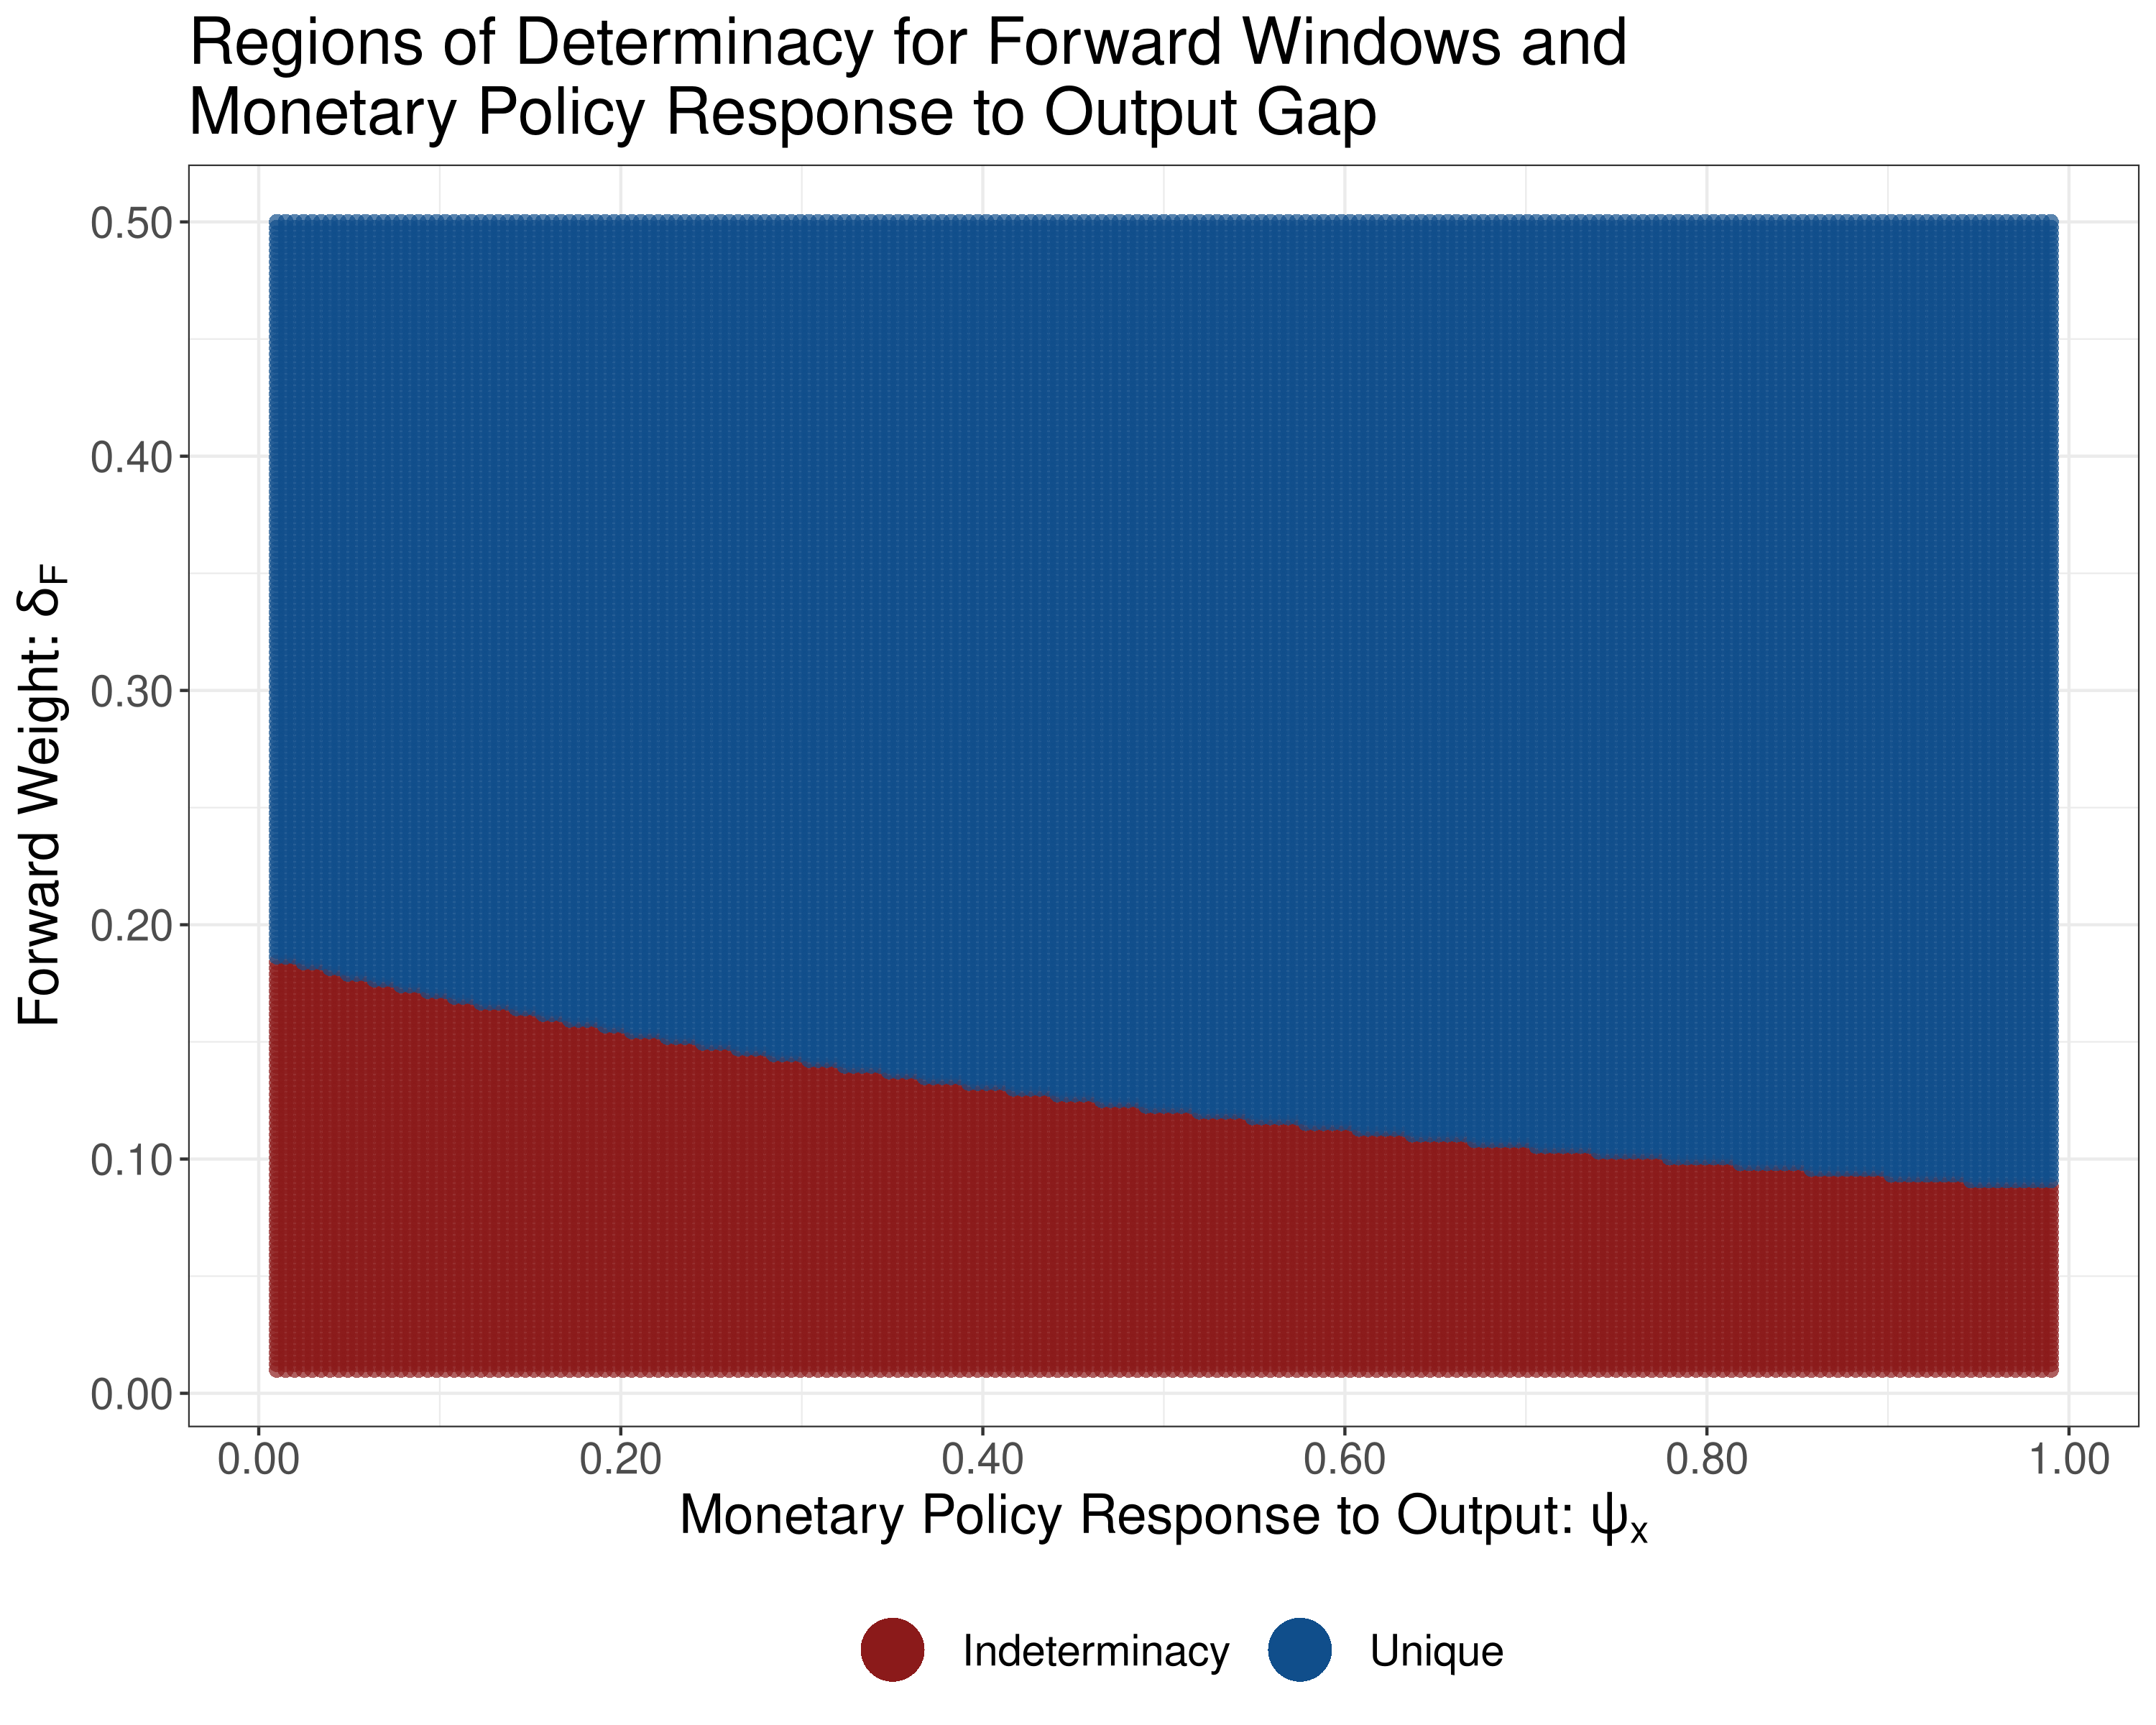
\includegraphics[width=\textwidth,height=0.6\textheight,keepaspectratio]{../code/psix_deltaF.png}
		\end{figure}% 
	\end{center}%
	\begin{enumerate}
		\setcounter{enumi}{5}
		\setlength{\itemsep}{1em}
		\item $\psi_x \geq 0.2$ is necessary for determinacy and larger values allow for longer forward windows.  
	\end{enumerate}
\end{frame}

\begin{frame}
	\frametitle{Varying the weight on policy persistence, $\rho_r$}	
	\begin{center}		
		\begin{figure}%
			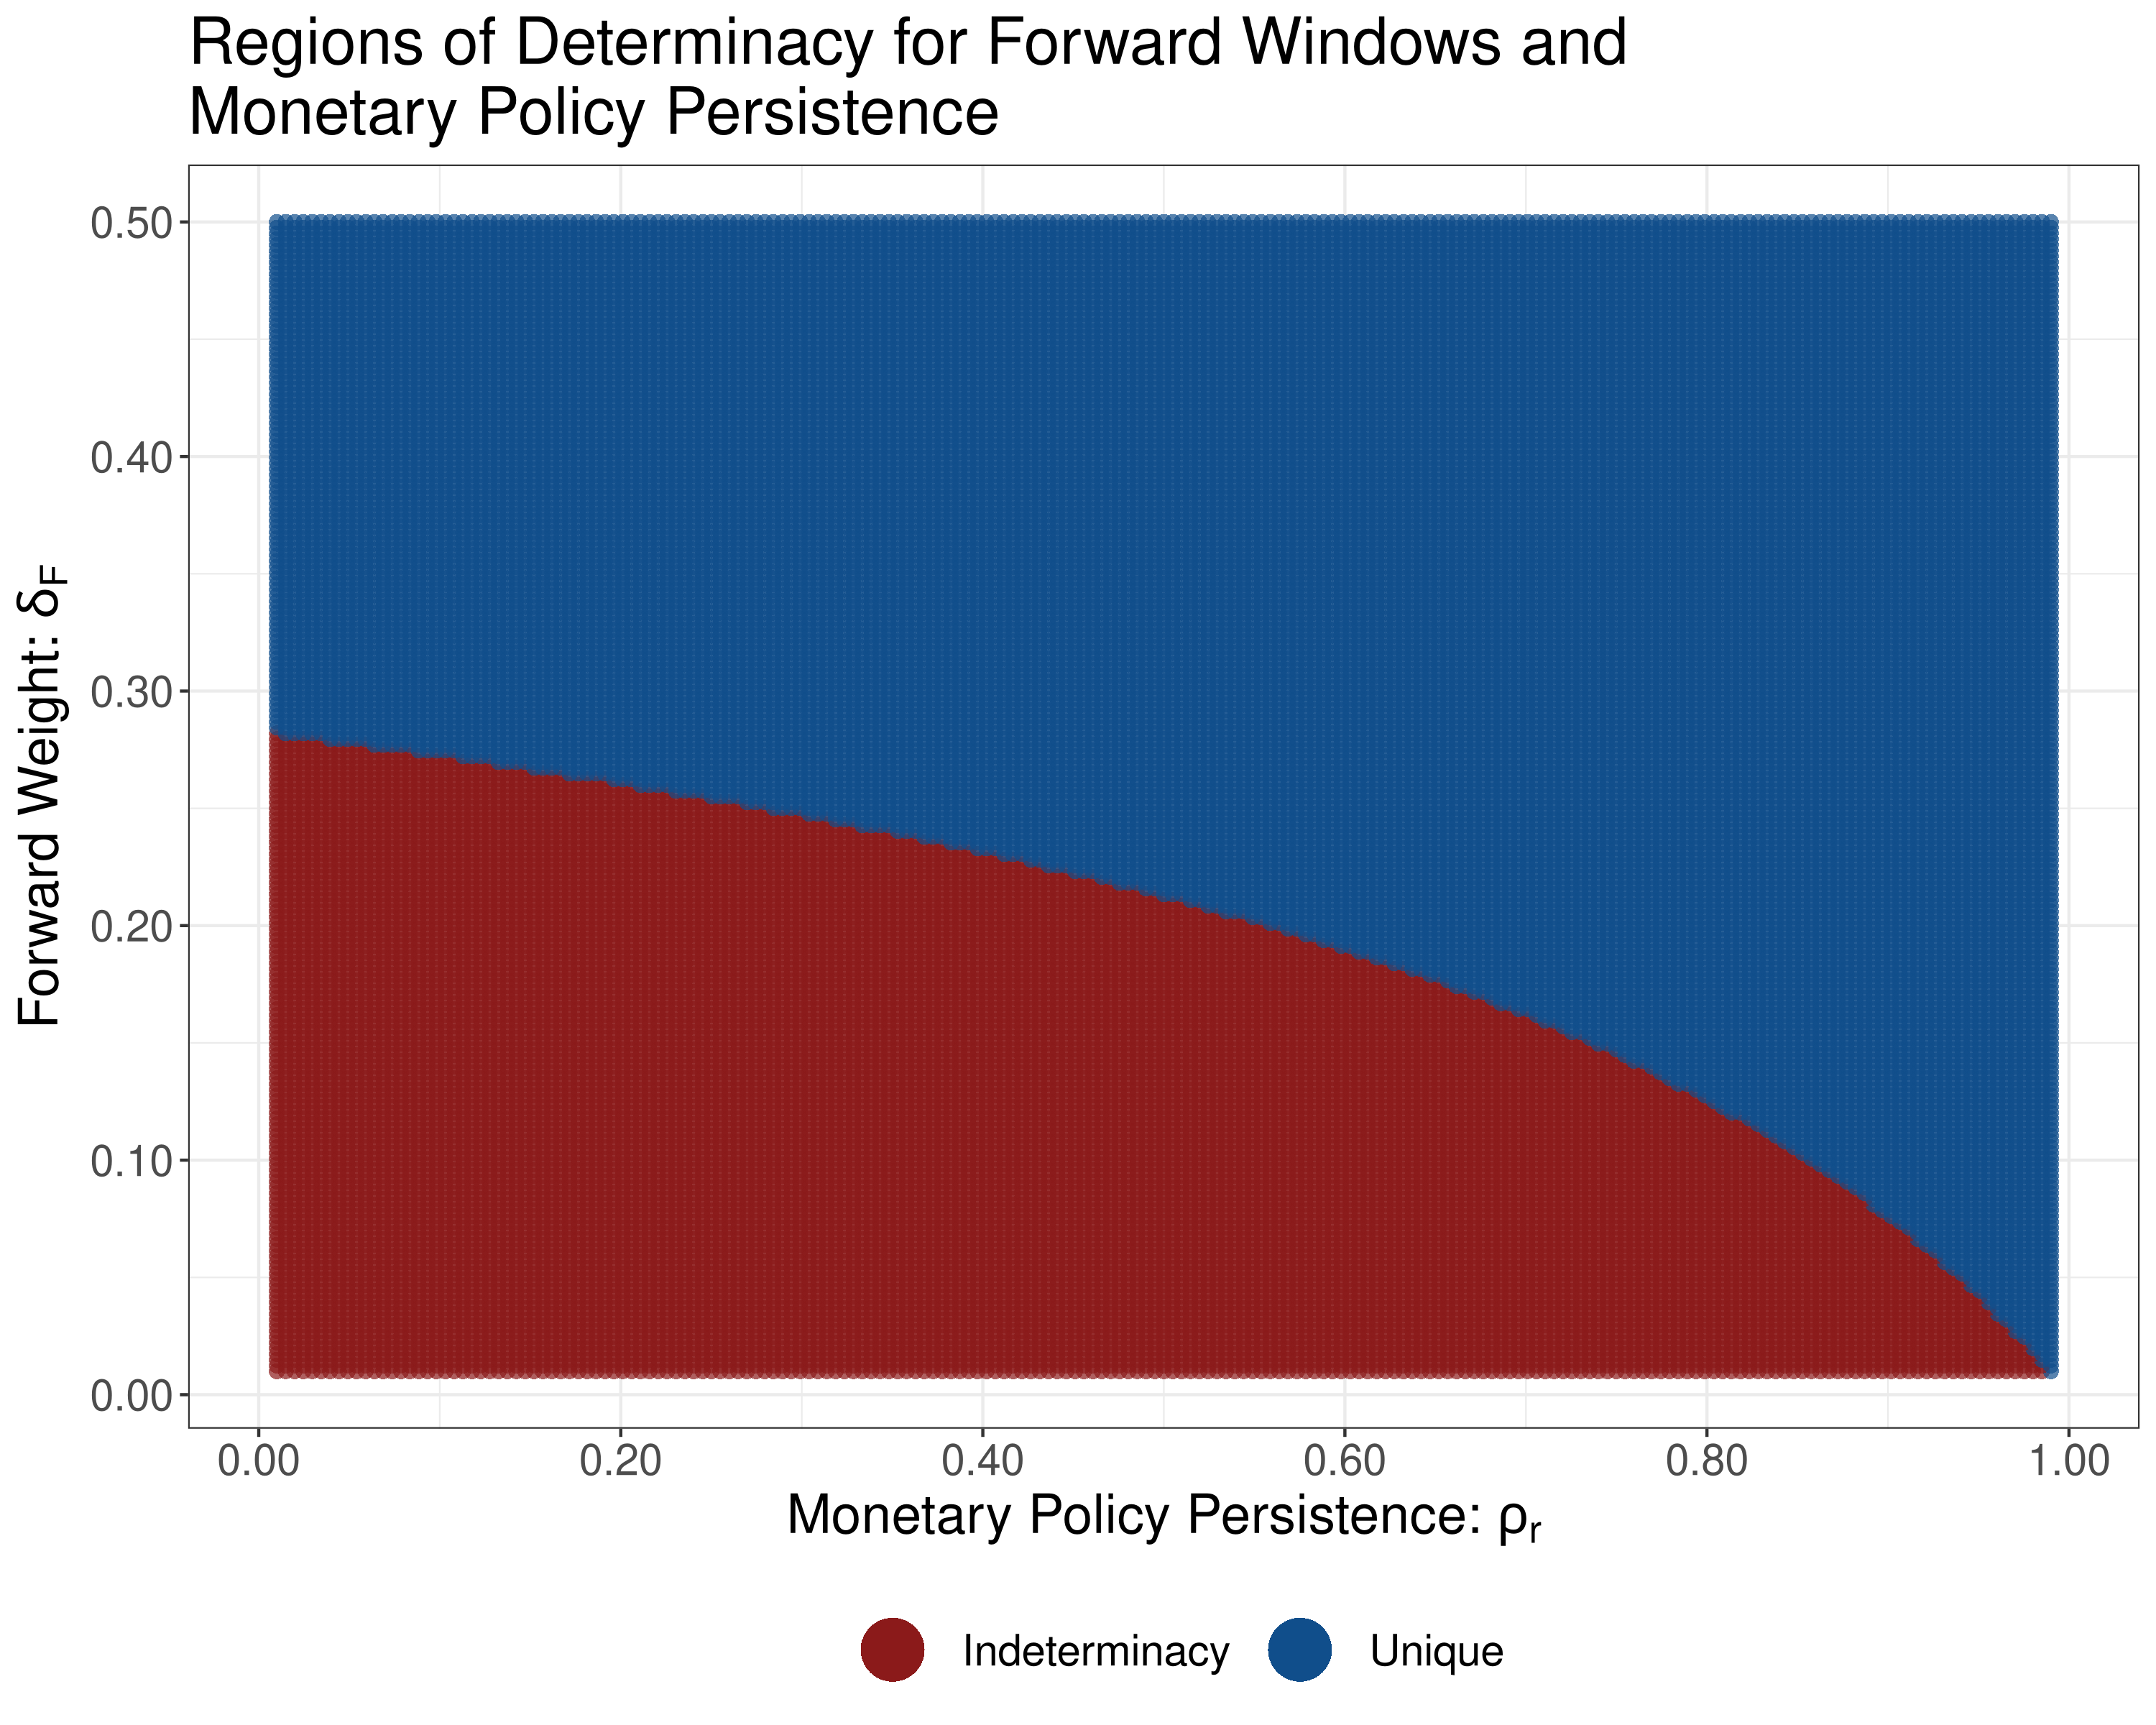
\includegraphics[width=\textwidth,height=0.6\textheight,keepaspectratio]{../code/rho_deltaF.png}
		\end{figure}% 
	\end{center}%
	\begin{enumerate}
		\setcounter{enumi}{6}
		\setlength{\itemsep}{1em}
		\item The stronger the persistence of monetary policy, the longer can be the forward looking window.  
	\end{enumerate}
\end{frame}

%\begin{frame}[allowframebreaks]
%	\frametitle{Summary of Results}
%	\begin{columns}
%		\begin{column}{0.5\textwidth}
%			\begin{enumerate}
%				\setlength{\itemsep}{1em}
%				\item In panel (A), $\delta_F =0.28$ is the smallest value that delivers determinacy in this scenario (the largest possible forward-looking window is approximately 3.57 quarters).
%				\item When $\gamma \geq 0.63$, all possible forward-looking windows yield determinate solutions. 
%				\begin{itemize}
%					\item This implies, though, that the target window has at least a 63\% weight on the current inflation rate, and therefore at most a 37\% weight on future inflation.
%				\end{itemize}
%			\end{enumerate}
%		\end{column}
%		\begin{column}{0.5\textwidth}
%			\begin{center}
%				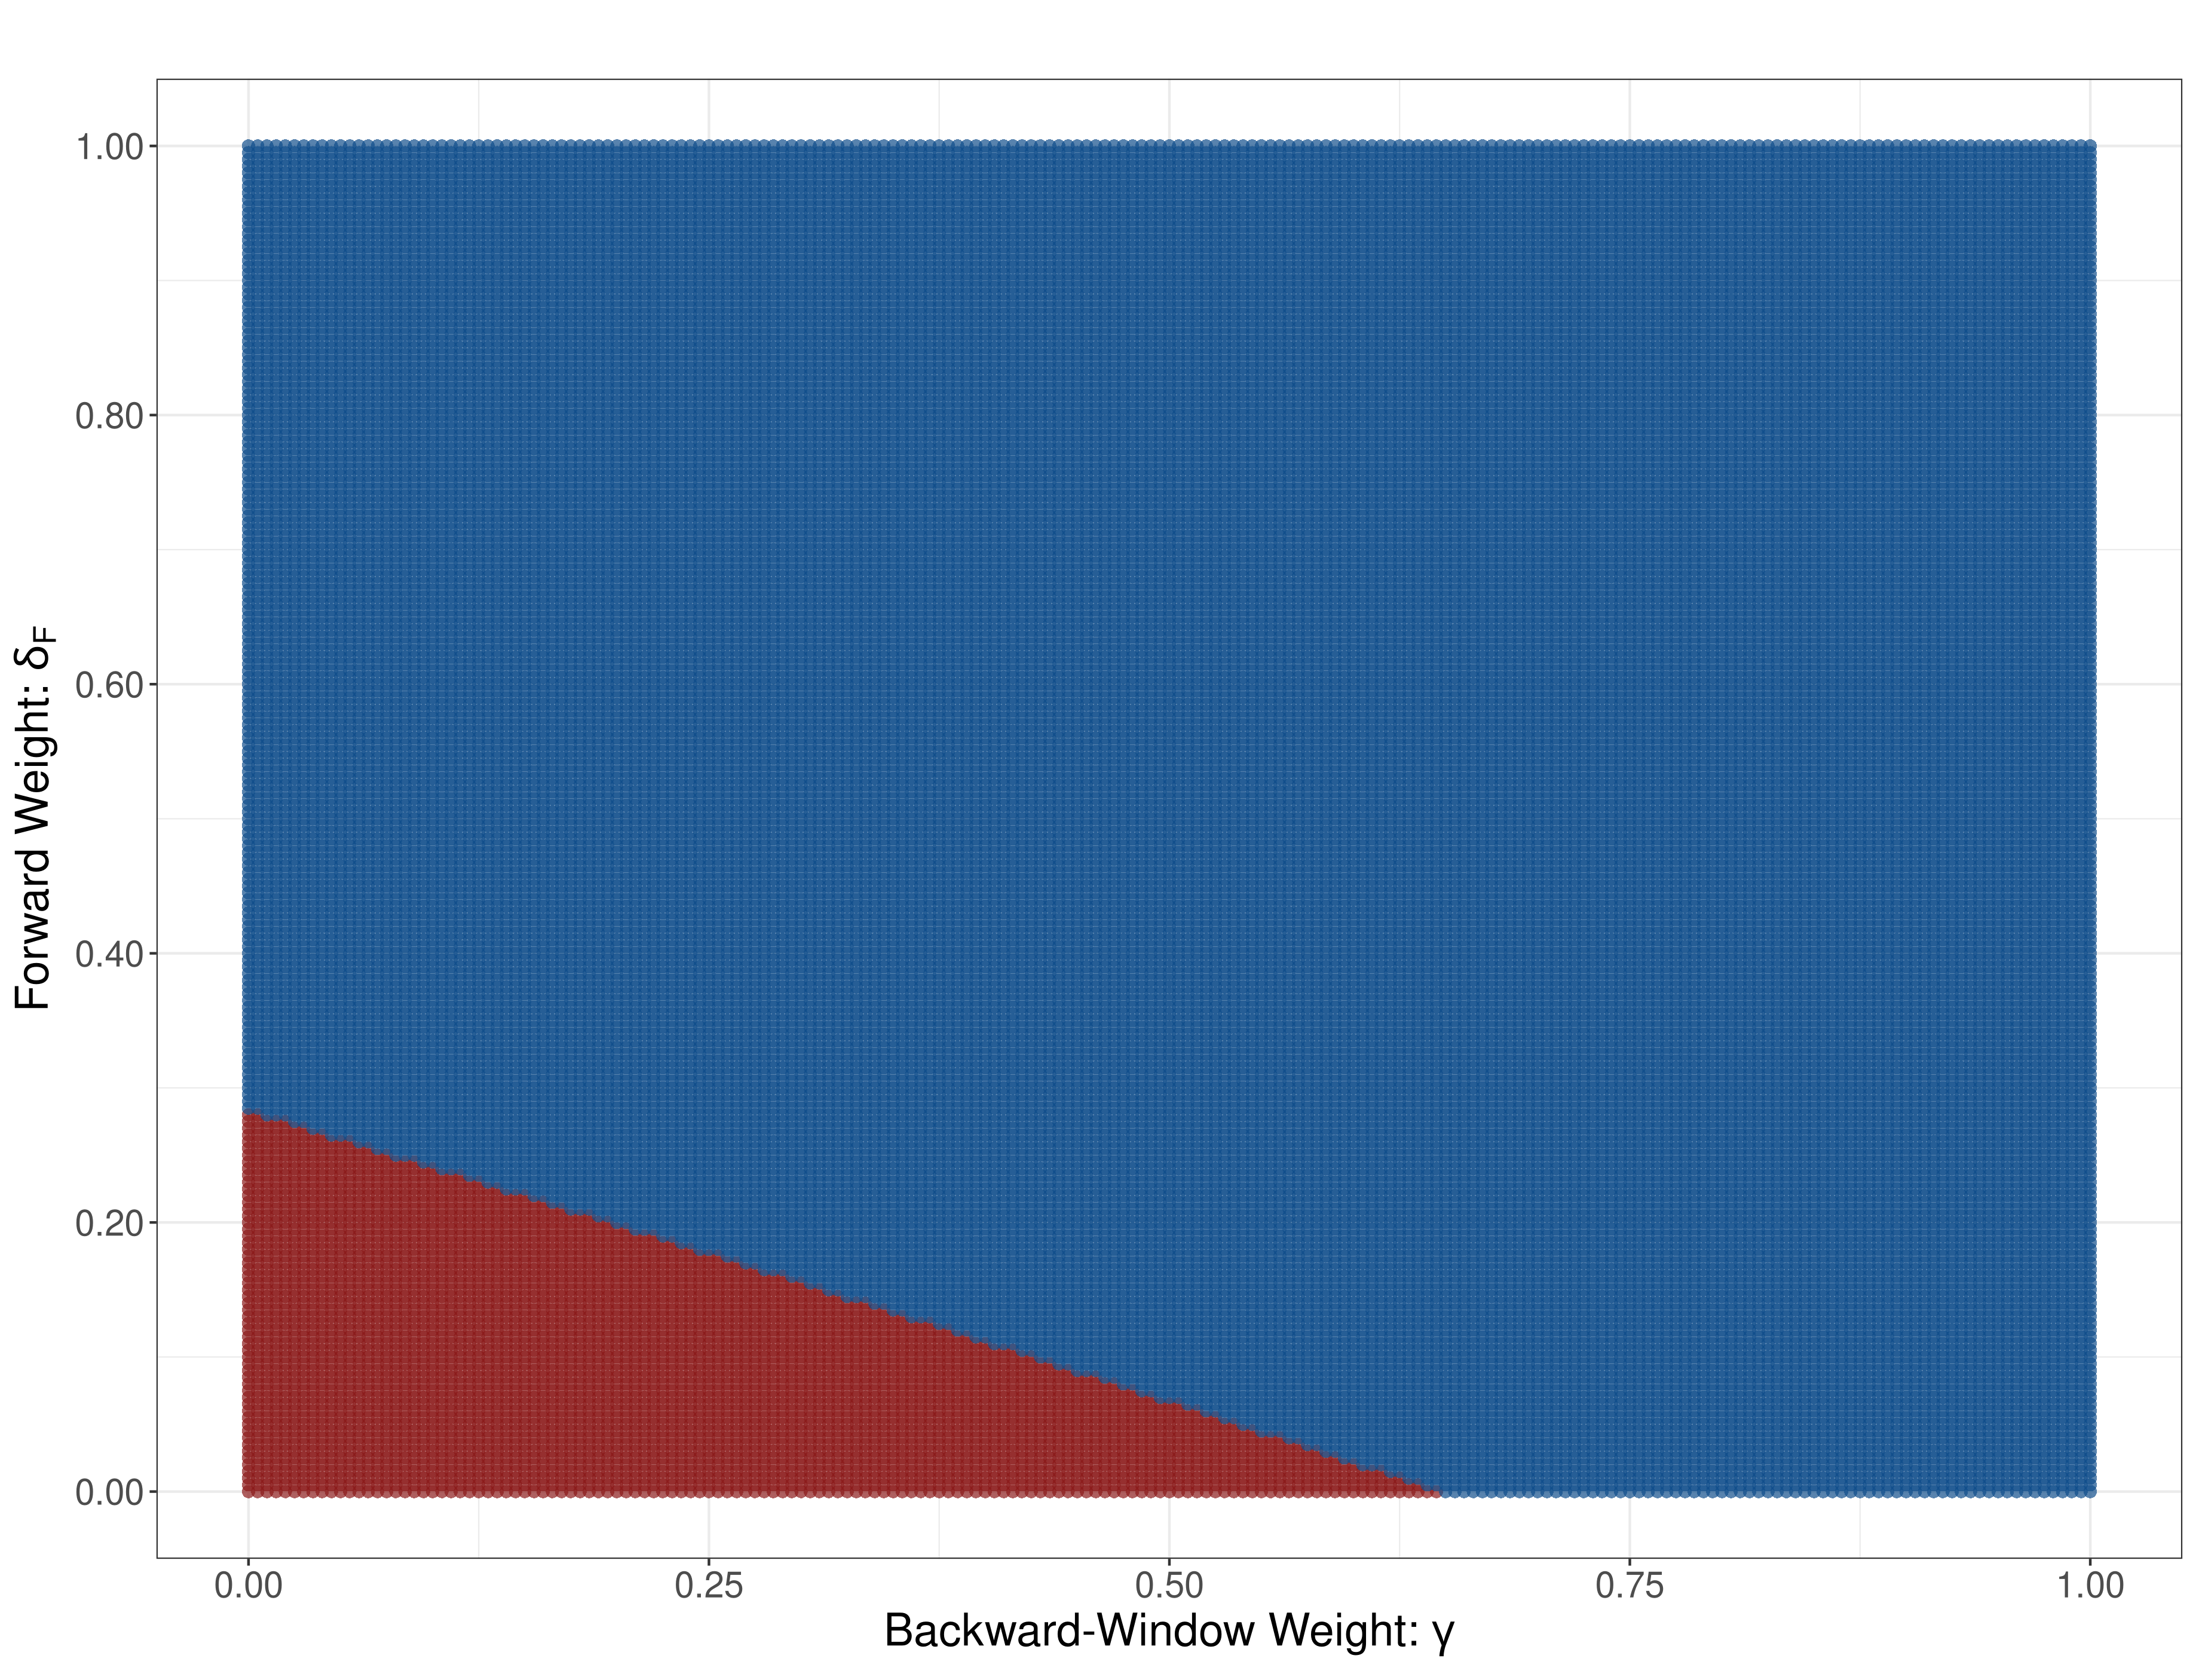
\includegraphics[width=\textwidth,height=\textheight,keepaspectratio]{../code/gamma_deltaF_notitle.png}
%			\end{center}
%		\end{column}
%	\end{columns}
%	
%	\begin{enumerate}
%		\setlength{\itemsep}{1em}
%		\item In panel (A), $\delta_F =0.28$ is the smallest value that delivers determinacy in this scenario (the largest possible forward-looking window is approximately 3.57 quarters).
%		\item When $\gamma \geq 0.63$, all possible forward-looking windows yield determinate solutions. 
%		\begin{itemize}
%			\item This implies, though, that the target window has at least a 63\% weight on the current inflation rate, and therefore at most a 37\% weight on future inflation.
%		\end{itemize}
%		\item In panel (B), the minimal combinations of values for $\delta_B$ and $\delta_F$ that achieve determinacy are each 0.14, implying the longest the forward-looking and backward-looking windows can be are approximately 7.14 quarters.
%		\item In panel (C), when more than 40\% of agents form na\"ive expectations, no purely forward-looking window for AIT leads to determinacy.
%		\item In general, larger response to inflation lead to more restrictive forward windows
%		\item $\psi_x \geq 0.2$ is necessary for determinacy and larger values allow for longer forward windows.  
%		\item The stronger the persistence of monetary policy, the longer can be the forward looking window.
%	\end{enumerate}
%\end{frame}

\begin{frame}
	\frametitle{Work to be done}
	\textcolor{purple}{Looking ahead ...}
	\begin{itemize}
		\setlength{\itemsep}{1em}
		\item Explore the rank condition to see what/how causes system to change from determinate to indeterminate (and vice versa) as model parameters change
		\item Impact of a monetary policy shock under AIT
		\item Impact on central bank credibility (crediblity/price shocks)
		\item Are there thresholds on how far a central bank can deviate from the long run target (... before monetary policy becomes time-inconsistent)?
	\end{itemize}
\end{frame}

\begin{frame}
	\centering
	The End! \\
	Thank you for your questions and comments.
\end{frame}

\appendix
\begin{frame}[allowframebreaks]
	\frametitle{References}
	\bibliographystyle{apalike}
	\bibliography{./ait_presentation.bib}
\end{frame}

\end{document}
